%!LW recipe=pdflatex ➞ bibtex ➞ pdflatex`×2

\documentclass{report}

\newcommand{\mytitle}{Building and Validating A Gaze-Aware AI System for Automatic Paragraph-Level Bookmarking}
\newcommand{\myauthor}{Henry Ash Williams}
\newcommand{\mydate}{\today}

\title{\mytitle}
\author{\myauthor}
\date{\mydate}

\usepackage[backend=bibtex]{biblatex}
\usepackage[compact]{titlesec}
\usepackage{kpfonts}
\usepackage[margin=2cm]{geometry}
\usepackage{hyperref}
\usepackage{siunitx}
\usepackage{graphicx}
\usepackage[super]{nth}
\usepackage{tabularx}
\usepackage{ltablex}
\usepackage{subcaption}
\usepackage{longtable}

\addbibresource{references.bib}

\begin{document}

\begin{titlepage}
    \begin{center}
        \vspace*{4cm}
        {\huge\textbf{\mytitle}}

        \vspace*{1cm}

        {\Large\textbf{\myauthor}

        \vspace*{0.75cm}

        \mydate}

        \vspace*{2cm}

        
\includegraphics[scale=0.075]{../assets/UoS-logo.png}

        \vspace*{2cm}

        {\Large BSc Computer Science with AI }

        \vspace*{2cm}

        {\large School of Engineering and Informatics

        Supervisor: Dr Temi Olugbade}
    \end{center}
\end{titlepage}

\tableofcontents

\chapter{Introduction}
\label{chap:intro}
\noindent
When using a web browser, users often have to switch back and forth between tabs, for example, to cross-reference facts with other sources, or to control music playing in the background. However, having someone's focus switch between multiple web pages leads to them forgetting their place in a body of text, and then having to waste their time finding it again. My project seeks to solve this by developing a web browser extension, called FocusFlow that will automatically detect and highlight the paragraph the user was reading before they switched tabs. To achieve this, I will utilize a technique called Gaze Mapping. This technique typically uses a mix of both specialized hardware and machine learning models to predict where a user is looking on a screen. While these solutions can achieve a high level of accuracy, \(\ang{0.3}\) from the true 3D gaze direction vector under ideal conditions~\cite{tobiiprofusion}, they require users to buy specialized, and often expensive equipment.

To make this technology more accessible, I aim to create a more cost-effective solution. My approach will make use of the existing cameras found in most modern devices, such as the webcam found in laptops, and front-facing cameras found in smartphones. Thus enabling us to extend the benefits of this technology to a broader audience. Several approaches for web-cam-based gaze mapping, otherwise known as appearance-based gaze mapping, have been proposed, but so far, none have been implemented into a browser extension. 

This report will outline the ethical considerations I made throughout development, Section~\ref{chap:ethics}, the background research I looked at which was necessary to develop my solution in Section~\ref{chap:background}, the design of my browser extension,~\autoref{chap:design} including an in-depth analysis of the requirements, the implementation detail of the browser extension, Section~\ref{chap:methods}, an evaluation of how well the browser extension meets the objectives outlined in Sections~\ref{sec:specific-objectives}~, ~\ref{sec:stretch-objectives}~\& which will be covered in Section~\ref{chap:results}, and finally a discussion of further work that could improve my the browser extension. 


\section{Motivation}

This project is motivated by the fact that there is no good way to automatically keep track of where you are in a large piece of text on digital devices.

My project seeks to solve this problem by visually showing users their place in the text, utilizing AI and machine learning.

The target user for this project is an individual who frequently reads on their computers and faces the challenge of losing their place in the text when switching tabs which can disrupt their workflow.

\section{Specific Objectives}\label{sec:specific-objectives}

There are two specific tasks I want to accomplish as part of this project. I have elaborated further on these objectives in \autoref{sec:requirement-analysis}, where I have performed an in-depth requirement analysis. 

\begin{itemize}
    \item The development and evaluation of a machine learning model that predicts the location of a user's gaze on a screen using images taken from their front-facing camera. The machine learning model should be able to make predictions within an approximate \(2.5\text{cm}\)~radius of the true gaze location, to accurately distinguish between paragraphs on the screen.
    \item This project is the development and validation of software that takes pictures from the user's webcam whenever the current browser tab is taken out of focus, securely transmits the image to another application hosting the aforementioned machine learning model and uses the model prediction to highlight the paragraph the user was reading last.
\end{itemize}

\section{Stretch Objectives}\label{sec:stretch-objectives}

Stretch objectives are tasks that I consider to be optional. If I have achieved my main goals, as outlined in Section~\ref{sec:specific-objectives}, and still have time before the final due date of the project, I will attempt to implement them.

\begin{itemize}
    \item A more accurate machine learning model, achieving an average accuracy of \(1\text{cm}\) of the true gaze location, enabling more accurate detection of paragraphs and could even be used to detect the reader's place in the text on a per-line or even per word basis.

    \item As it currently stands, the locations of the paragraphs will be detected using the information provided by the document object model (DOM) of the webpage. However, I want this extension to work on documents that aren't written in HTML, such as PDFs. This would require a computer vision system to detect where paragraphs are in an image.
\end{itemize}

\chapter{Professional and Ethical Considerations}
\label{chap:ethics}

\noindent
The BCS code of conduct \cite{bcs2022coc} outlines a set of guidelines which IT professionals are expected to follow. These guidelines seek to improve the public image of ethical practices within the computing field. They include considerations relating to the interest of the public, professional competence and integrity, duty to the relevant authorities and the profession. This section will explore how I will ensure my project adheres to these guidelines. 

\section{Public Interest}   

In order to adhere to the requirements set out by BCS, my project must ensure that the health, privacy, security and well-being of its users are respected. 

To ensure the privacy of users is respected, the software will not share any information with third parties and will be fully encrypted while in transit between the web browser and the machine learning model. 

Furthermore, the images captured to facilitate gaze mapping will not be stored, and instead will immediately be discarded once they have been used by the machine learning model to predict their gaze location.

Users will be in complete control of the capture of these images and will be informed as to how the images will be used. However, if the user does not grant the application permission to use their device's camera, the extension will not function. 

To ensure the machine learning model behaves as expected for all users, the model will be trained on a diverse set of participants. The datasets I plan on using however include over 1500 unique participants, made up of people with diverse backgrounds. This should ensure the model learns how to function correctly for all users. 

The software will be freely available for all of the most commonly used browsers. This includes Google Chrome, Firefox, Microsoft Edge, and Opera. 

\section{Professional Competence \& Integrity}   

Section two of the BCS code of conduct outlines requirements relating to the professional competence and integrity of the person developing the software. The first three points within this section state that the project should be within your level of expertise, that you should not claim any level of competence that you do not possess, and that you should develop your skills and competence as part of the project. I have discussed my project with my supervisor, and we believe that this project is within my professional competence.

I have also researched the relevant legislation regarding user data and machine learning models, and will not violate any such legislation as part of this project. 

The code of conduct also states that alternative viewpoints and honest criticism of work are respected and valued. I plan on regularly meeting with my supervisor to gain insight into my project and gather feedback as to how to improve. 

I also understand that I must avoid injuring others, their property, reputation or employment by malicious or negligent action or inaction. This includes respecting the rights of the authors of the datasets which I plan on using, and their participants. Every action I can possibly make to ensure their rights are respected will be taken. 

Finally, I will not take or make bribes behave in unethical practices, and discourage other professionals from similar actions.  

\section{Duty to Relevant Authority}   

The project will be developed with the utmost care and respect for the academic policies of the University of Sussex. This includes avoiding potential conflicts of interest and accepting responsibility for any that may arise during development. No confidential information will be disclosed without explicit permission of the University. Furthermore, no information will be misrepresented or withheld. 

\section{Duty to the Profession}   

As part of my duty to the profession, I commit to upholding the reputation of the profession by accepting personal responsibility and will ensure that no actions will harm its standing. This project will be dedicated to taking positive steps to enhance the professional standards of the profession and actively contributing to upholding the reputation of BCS. I will conduct myself with integrity and respect in all professional relationships with BCS members and others. Furthermore, I will be committed to fostering a supportive environment by encouraging and assisting others to uphold the same goals. 

\chapter{Background and Related Works}
\label{chap:background}
\noindent
In recent years, eye tracking has emerged as a significant field of study within human-computer interaction and computer vision~\cite{cheng2021survey,kar2017review}. It offers engineers the ability to determine where a user is looking, allowing them to better understand how users interact with a system. Several techniques have been proposed for this task, such as 3D eye model recovery, appearance-based techniques, and 2D eye feature-based approaches. This section of the report will provide an overview of the gaze estimation landscape, how it relates to my project, and a background overview of the browser extension development landscape. 

\section{2D vs 3D Gaze Estimation} 

Depending on the domain, the output from a gaze estimation system can come in one of two forms~\cite{liu2022in}, a 3D gaze direction vector representing where in physical space a user is looking, or a 2D point-of-gaze representing where the user is looking on the screen. The former mostly being used to track users' attention and focus within a real-world environment, an example of such a task is an advertiser attempting to quantify how effective their advertisement is within a shop by measuring how much time on average a customer spends looking at it. By looking at the gaze direction, and the customer's position in the environment, the system can determine if their gaze is directed towards the advert, and record how long they have been looking at it, or how long it takes them to notice and look at the advertisement. 2D point of gaze, however, considers users' interactions with a computer. The point of gaze represents the approximate location of the user's gaze on a computer screen, such as a smartphone or laptop. This can be used for several tasks, such as hands-free computer interaction, and research considering how people interact with computers. 

These two methods of predicting gaze have each been researched extensively, and several approaches for each of them have been outlined. For 3D Gaze, techniques such as stationary, mobile, and even head-mounted devices have been proposed. For 2D point-of-gaze prediction, two primary approaches for capturing input images have emerged, namely making use of in-built cameras, such as the front-facing camera on a smartphone or the integrated webcam on a laptop, known as appearance-based gaze mapping, and specific hardware devices that make use of infrared imaging such as the devices manufactured by Tobii~\cite{tobiiprofusion} (a company which specializes in eye tracking for commercial and research purposes). 

However, it is worth noting that despite these approaches being the most prominent in the literature, other approaches have been proposed. For example, by attaching electrodes to the face of a user, it is possible to indirectly observe the movements of the eye~\cite{young1975survey} and then use this information to estimate both the location of the gaze target and the direction of gaze within a physical space. This approach has seen little development however as it requires the use of invasive electrodes mounted to the user's face, which is not ideal for a real-world application. 

My research considers an appearance-based 2D point of gaze prediction, as it provides my software with the necessary information to determine what the user is currently reading. 3D gaze direction-based models would be insufficient for the task at hand as they require additional information to convert the vector to a gaze target~\cite{cheng2021survey} such as the screen pose \(\{\pmb R_s, \pmb T_s\}\), and the origin \(o\). The screen pose captures the rotation matrix of the screen, \(\pmb R_s\), and the translation matrix, \(\pmb T_s\). To determine the values for each of these parameters, an extra step is required before gaze location prediction can occur; this could introduce inaccuracy into the system, thereby introducing more error into the overall system, and decreasing its overall effectiveness while increasing computational complexity. 

The input to my model is an image from the user's webcam, which provides a simple RGB image of the user's face. This has several benefits when compared to other approaches such as 2D feature regression and 3D eye model recovery methods, as they require a specialist infra-red camera to accurately map gaze location, and often aren't robust to changes in head pose~\cite{zhu2006nonlinear}. Appearance-based models learn a simple RGB image which is far easier to capture, as it does not require additional, and often specialized hardware, as many personal computing devices provide access to built-in front-facing cameras. 

\section{2D Point-of-Gaze Appearance-Based Deep Learning Models for Gaze Mapping}


One of the most promising, state-of-the-art models I discovered as part of my background research was the iTracker model proposed by~\textcite{krafka2016eye}. This model takes an RGB image from the user's integrated camera, crops the left and right eyes, and the face, and creates a binary mask showing where in the image the face is located and learns the 2D point-of-gaze on the computer screen, see~\autoref{fig:itracker-model}. It is based on the Convolutional Neural Network (CNN) architecture and has been shown to achieve excellent performance at performing inference across various domains~\cite{cheng2021survey}. The paper also outlines their Gazecapture dataset, which is a crowd-sourced dataset with approximately 1500 participants. 

\begin{figure}[h]
    \begin{center}
        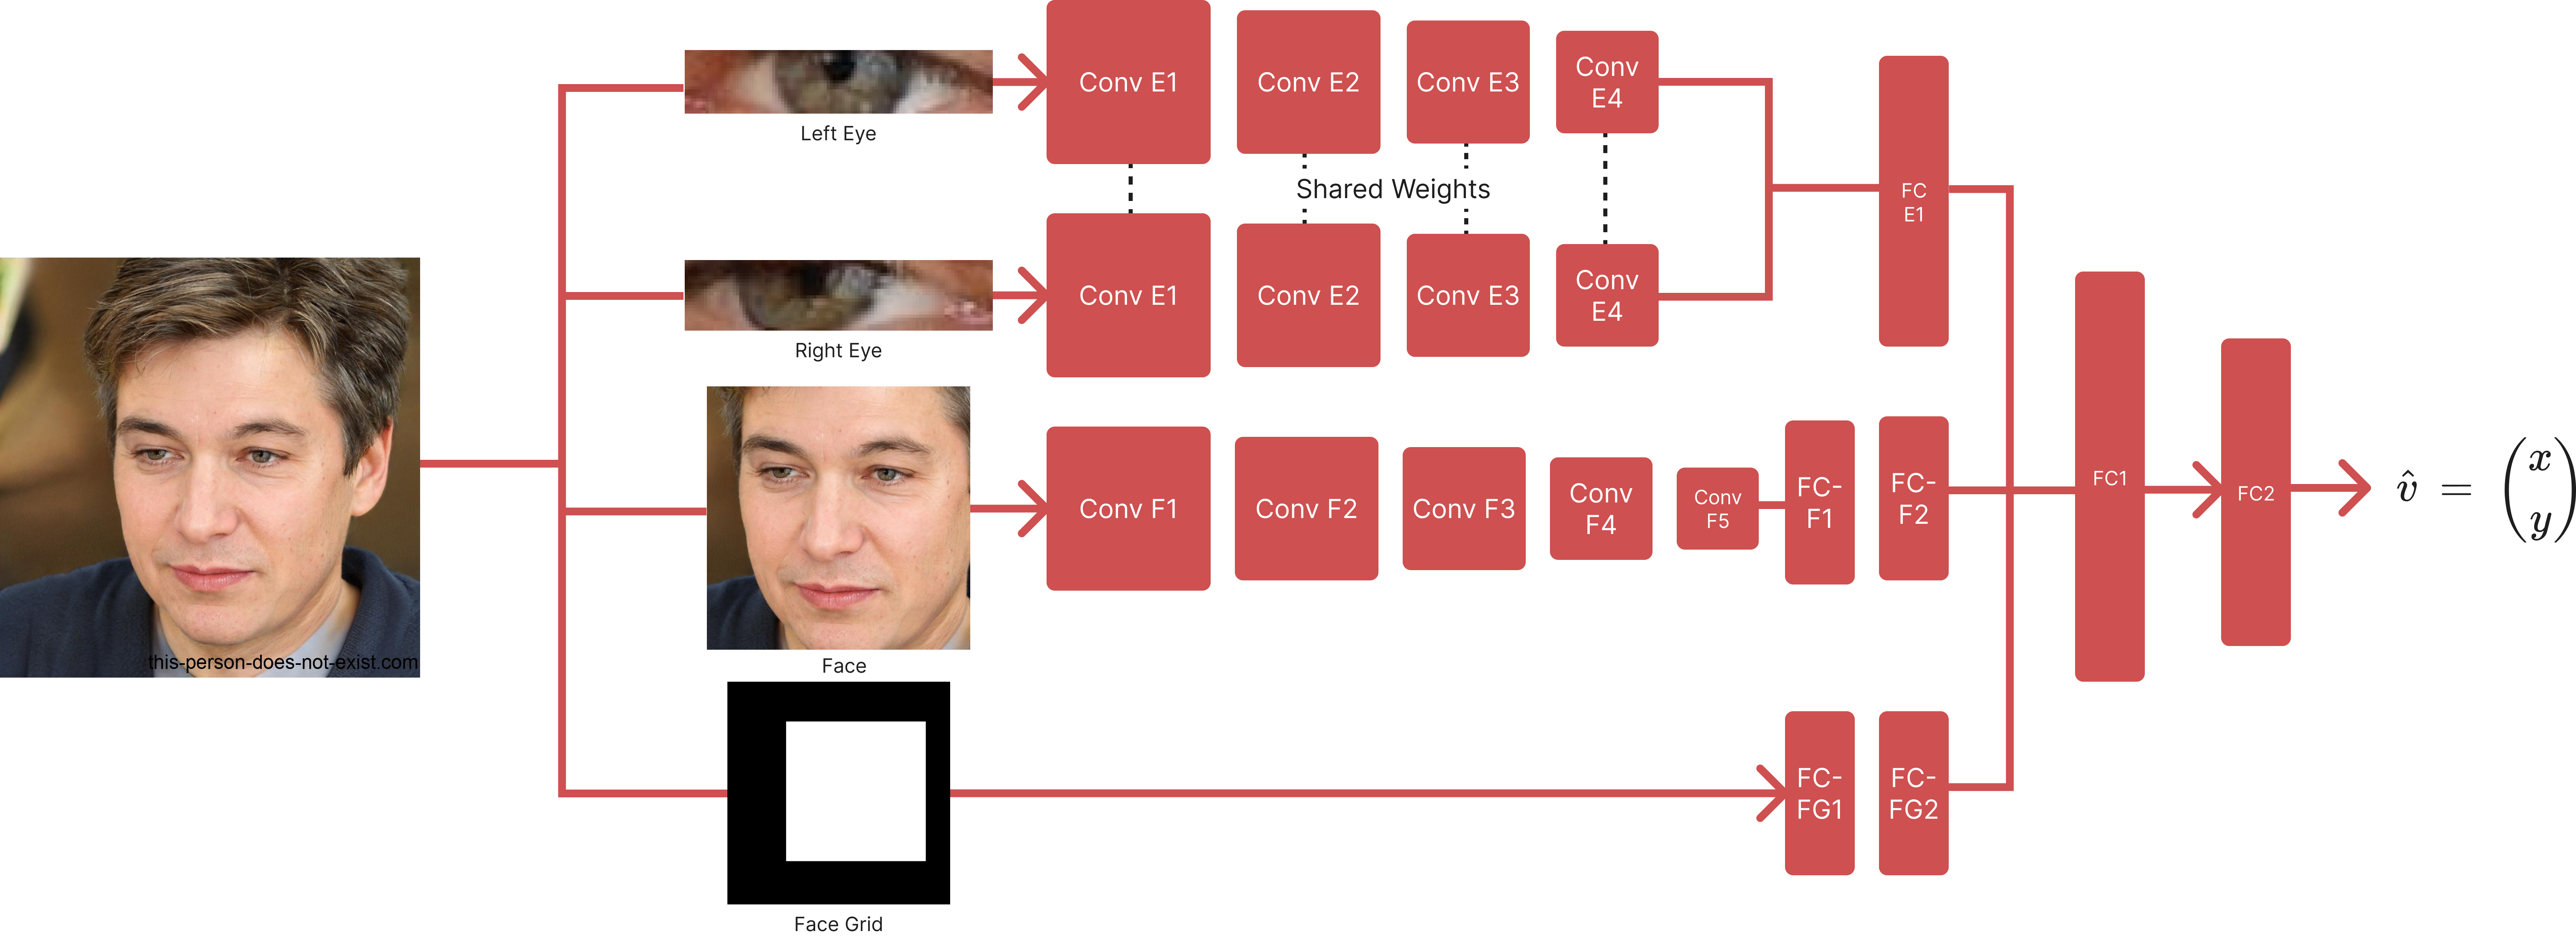
\includegraphics[scale=0.07]{../assets/itracker-model-my-own.png}
    \end{center}
    \caption{The structure of the iTracker model, \(0\leq x \leq 1,~0 \leq y \leq 1\)}
    \label{fig:itracker-model}
\end{figure}

The only issue with using iTracker trained on the Gazecapture dataset is that it was designed for gaze prediction on mobile devices. However, the repository~\cite{krafka2016eye,cheng2021survey} made available as part of their publication offered a configuration that allows the model to be trained on the MPII Face Gaze~\cite{zhang2019mpii} dataset, which captures the point of gaze information and images from people's laptops rather than phones as the Gazecapture dataset does.

In the final release of my software, it will need to work on both mobile and desktop devices. I plan on training two models, one for clients on desktop devices and another for mobile devices.

In the literature, researchers highlight the importance of calibration for increased gaze mapping accuracy. Seonwook Park's (et al\.) paper~\cite{seonwook2019fewshot} explains why this additional step is necessary for high-accuracy gaze mapping models, and introduces their FAZE (Few-shot Adaptive GaZE Estimation) framework which seeks to create a specialized model for a given user with a few shot approach. By training a generalized model on a few calibration points, their approach demonstrates significantly improved accuracy when compared to the generalized model. 

I also looked at several other approaches for gaze estimation using a CNN, and I found that most state-of-the-art approaches, such as AFF-Net~\cite{bao2021adaptive}, SAGE~\cite{junfeng2019on}, and EFE~\cite{balim2023efe} had similar approaches to iTracker, with similar results across domains. For example, AFF-Net made use of the eye and face cropping technique proposed by iTracker. 

To decrease training time, I looked into the performance of pre-trained CNNs for this technique, such as AlexNet~\cite{krizhevsky2017imagenet} and RES-Net~\cite{deng2009imagenet}. This is a well-researched approach for image-based deep-learning tasks, where a pre-trained model is fine-tuned on a new task. The benefit of using this approach, known as transfer learning allows researchers to cut down on both time spent training and the size of the dataset used to train the model. However, when compared to the performance of specialized architectures, their performance is worse. For example, when trained on the MPII Gaze dataset, AlexNet achieved a test error of \(4.8\text{cm}\) whereas the architecture proposed by~\textcite{akinyelu2020convolutional} was able to achieve \(4.6\text{cm}\) test error.

\section{Browser Extension Background}\label{sec:browser-extension-background}

Browser extensions allow users to modify the behaviour of their web browser. There are several reasons why a user might want to install a browser extension. From improving the accessibility of webpages by changing their appearance and making use of ARIA tags~\cite{w3c2018accessible,lsdsoftware2024read}, improving security through the use of password managers, enabling users to generate and store secure passwords linked to a specific website and inserted into password fields automatically~\cite{lastpass}, to ad blocker extensions which hide advertisements on webpages~\cite{hill2014ublock}, and even access the digital currency wallets of users~\cite{finlay2015metamask}. These extensions run on top of the page and allow developers to interact with almost every aspect of the page~\cite{frisbe2022building}, including network requests, and the Document Object Model (DOM).

The document object model represents an HTML document as a tree, which can be manipulated by JavaScript. This is a very powerful concept that has largely been responsible for the rise of dynamic web pages, also known as Web 2.0. Browser extensions can interact with, and manipulate this tree in any way they see fit, enabling developers to customise the behaviour of websites. Browser extensions can access the DOM using an API provided by the browser. 

Browser extensions were first introduced by Microsoft's Internet Explorer in 1999. In the early days of browser extensions, developers had to make use of proprietary APIs that were limited to a single browser. Thus, a distinct codebase was required for each browser they wanted the extension to be available on. In 2009, Google Chrome introduced a new API for developing browser extensions that allowed them to be written in languages such as HTML, CSS, and Javascript; the same languages used to write websites. When Google Chrome rapidly became the most popular browser in 2012, other browsers implemented their API for their platform, and quickly became the standard API for developing browser extensions. This enabled developers to use a single codebase for an extension across multiple browsers. 

In every browser extension, there is a file known as the manifest. This file contains the metadata for the extension in the JavaScript Object Notation (JSON) format and includes keys such as author, background scripts, and a description of the extension behaviour~\cite{bengtsson2020manifest}. In 2020, the chromium developer team announced a new version of this file, known as manifest V3. This update provided many improvements to security, performance, and privacy~\cite{li2020manifest,}. However, part of this update limited developers' access to network requests which many browser extensions rely on. Manifest V3 also forces all extensions to contain all of their functionality within the extension itself, for example, the extension cannot load and execute remotely hosted files. These changes were very controversial, as many saw it as an attempt to hinder the effectiveness of ad-blockers~\cite{barnett2021chrome}, and browsers based on alternative engines such as Firefox announced that they would not depreciate the existing Manifest V2 API, while still allowing extensions to use the new Manifest V3 API.  

\subsection{AI in the Browser}\label{ssec:ai-in-the-browser}

With the recent explosion of AI for commercial purposes, many developers have wanted to integrate these platforms into their web applications. As it stands, the most common approach to this task is to remotely host deep learning models on a remote server and to communicate with them over an architecture such as REST~\cite{fielding2000phd}. This is likely because machine learning models are often very large, and require a lot of computational resources to perform their inferences. Therefore, users with slow internet connections, or weak hardware would struggle to use them. Developers instead opt to remotely host these models, on powerful hardware provided by cloud platforms such as Amazon Web Services (AWS). However, it is worth noting that machine learning models can be hosted on the client side of a web browser thanks to frameworks such as TensorFlow.js~\cite{tensorflow2015whitepaper}, and ONNX.js~\cite{onnxruntime}, despite this, performing inference in the browser can significantly impact performance~\cite{yun2019moving}. 

% For this reason, I've decided to make use of a REST API, as outlined by Fielding in his PhD dissertation~\cite{fielding2000phd} to offload the task of performing inference to the user's local machine instead of the browser. This enables us to make use of the user GPU (if present), and CPU multithreading, which many of the browser-side machine-learning frameworks lack support for. 


\chapter{Design}
\label{chap:design}

In this chapter, I will introduce the design considerations of both my web browser extension and the machine learning model alongside the requirements, user interface, and system flow of the browser extension, and the machine learning model. 

\section{Requirement Analysis}\label{sec:requirement-analysis}

While I introduced some requirements as part of my introduction, these were vague and insufficient from a software design perspective. This section should remove all ambiguity regarding what this browser extension requires to function.  


\subsection{Functional Requirements}

Functional requirements describe what the web browser extension should do. This includes how and where the browser extension should run and the objectives of the machine learning model.

\begin{itemize}
    \item The browser extension must run on as many possible browsers as possible, including all of the most popular such as Chrome, Firefox, Edge, and UC browser. 
    \item The browser extension must request permission from the user to access their integrated camera.
    \item The browser extension must highlight the paragraph that they were last reading before the page went out of focus. 
    \item The browser extension must be able to determine the platform it's currently running on, i.e.~mobile, or desktop. 
    \item The browser extension must securely transmit the images taken from the web page to the API 
    \item The machine learning model must predict the location of the user gaze within approximately \(2.5\text{cm}\) of the user's location gaze 
    \item The machine learning model must work in a variety of lighting conditions.
    \item The machine learning model must work with a variety of head poses. 
    \item The machine learning model must work on devices with a variety of screen sizes 
    \item The user must be able to configure how the browser extension highlights paragraph elements 
    \item The web browser should work on both mobile and desktop browsers. 
\end{itemize}

\subsection{Non-Functional Requirements}

Non-functional requirements outline criteria that can be used to judge the effectiveness of the browser extension. 

\begin{itemize}
    \item The machine learning model must not be biased, i.e.~it works only for caucasian users. 
\end{itemize}

\subsection{Stretch Requirements}\label{ssec:stretch}

Should I have time to continue development after achieving my main objectives outlined above, I have devised several stretch objectives that would further enhance the performance and usefulness of my browser extension. 

My first stretch objective is to see if it is possible to bookmark the reader's position on a line-by-line basis or even a word-by-word basis. This would allow the browser extension to better track where on the page a user is reading. It could also have implications for the development of accessibility tools for users with attention disorders or reading difficulties. For example, in the case of readers with dyslexia, showing the text on a line the user is currently reading, and blocking everything else out on the text, has been shown to drastically improve reading comprehension~\cite{mutalib2022student}. This is a stretch objective as the line height of a body of text is usually very small, around 0.5cm, meaning the model would have to be capable of predicting gaze within this very small radius. The model I selected to perform gaze inference can achieve a test error of around 2cm on mobile devices and around 8cm on desktop devices. Therefore, achieving this stretch objective would likely require selecting and training, or even developing my own model capable of fulfilling this extremely difficult requirement. However, this model could be used to develop future browser extensions that could massively improve the accessibility of the web for users with different needs. 

Another of my stretch objectives is to develop a computer vision system to automatically detect the location of paragraphs in text. My current approach for the browser extension makes use of the semantic information offered by the HTML document to detect where paragraphs are on a page. For example, any element with the \texttt{<p>} tag is a paragraph, and I can easily get the bounding box of this element using the \texttt{HTMLElement.getBoundingClientRect()} method, which returns two tuples representing the top-leftmost and bottom-rightmost location of a rectangle containing the entire HTML element. However, not all pages visited on a web browser are defined in HTML, for example, pdfs, images, and plain text files. Therefore, my approach would not work for these files and another approach is necessary. By developing a computer vision system to create a binary mask showing where there are paragraphs in the image such as in~\autoref{fig:binary-mask}, the browser extension can use this information to check where the location of gaze intersects with a paragraph, which can then be highlighted on the page. This would enable the browser extension to function on a variety of files that may be displayed on a web browser. 

\begin{figure}
    \centering
    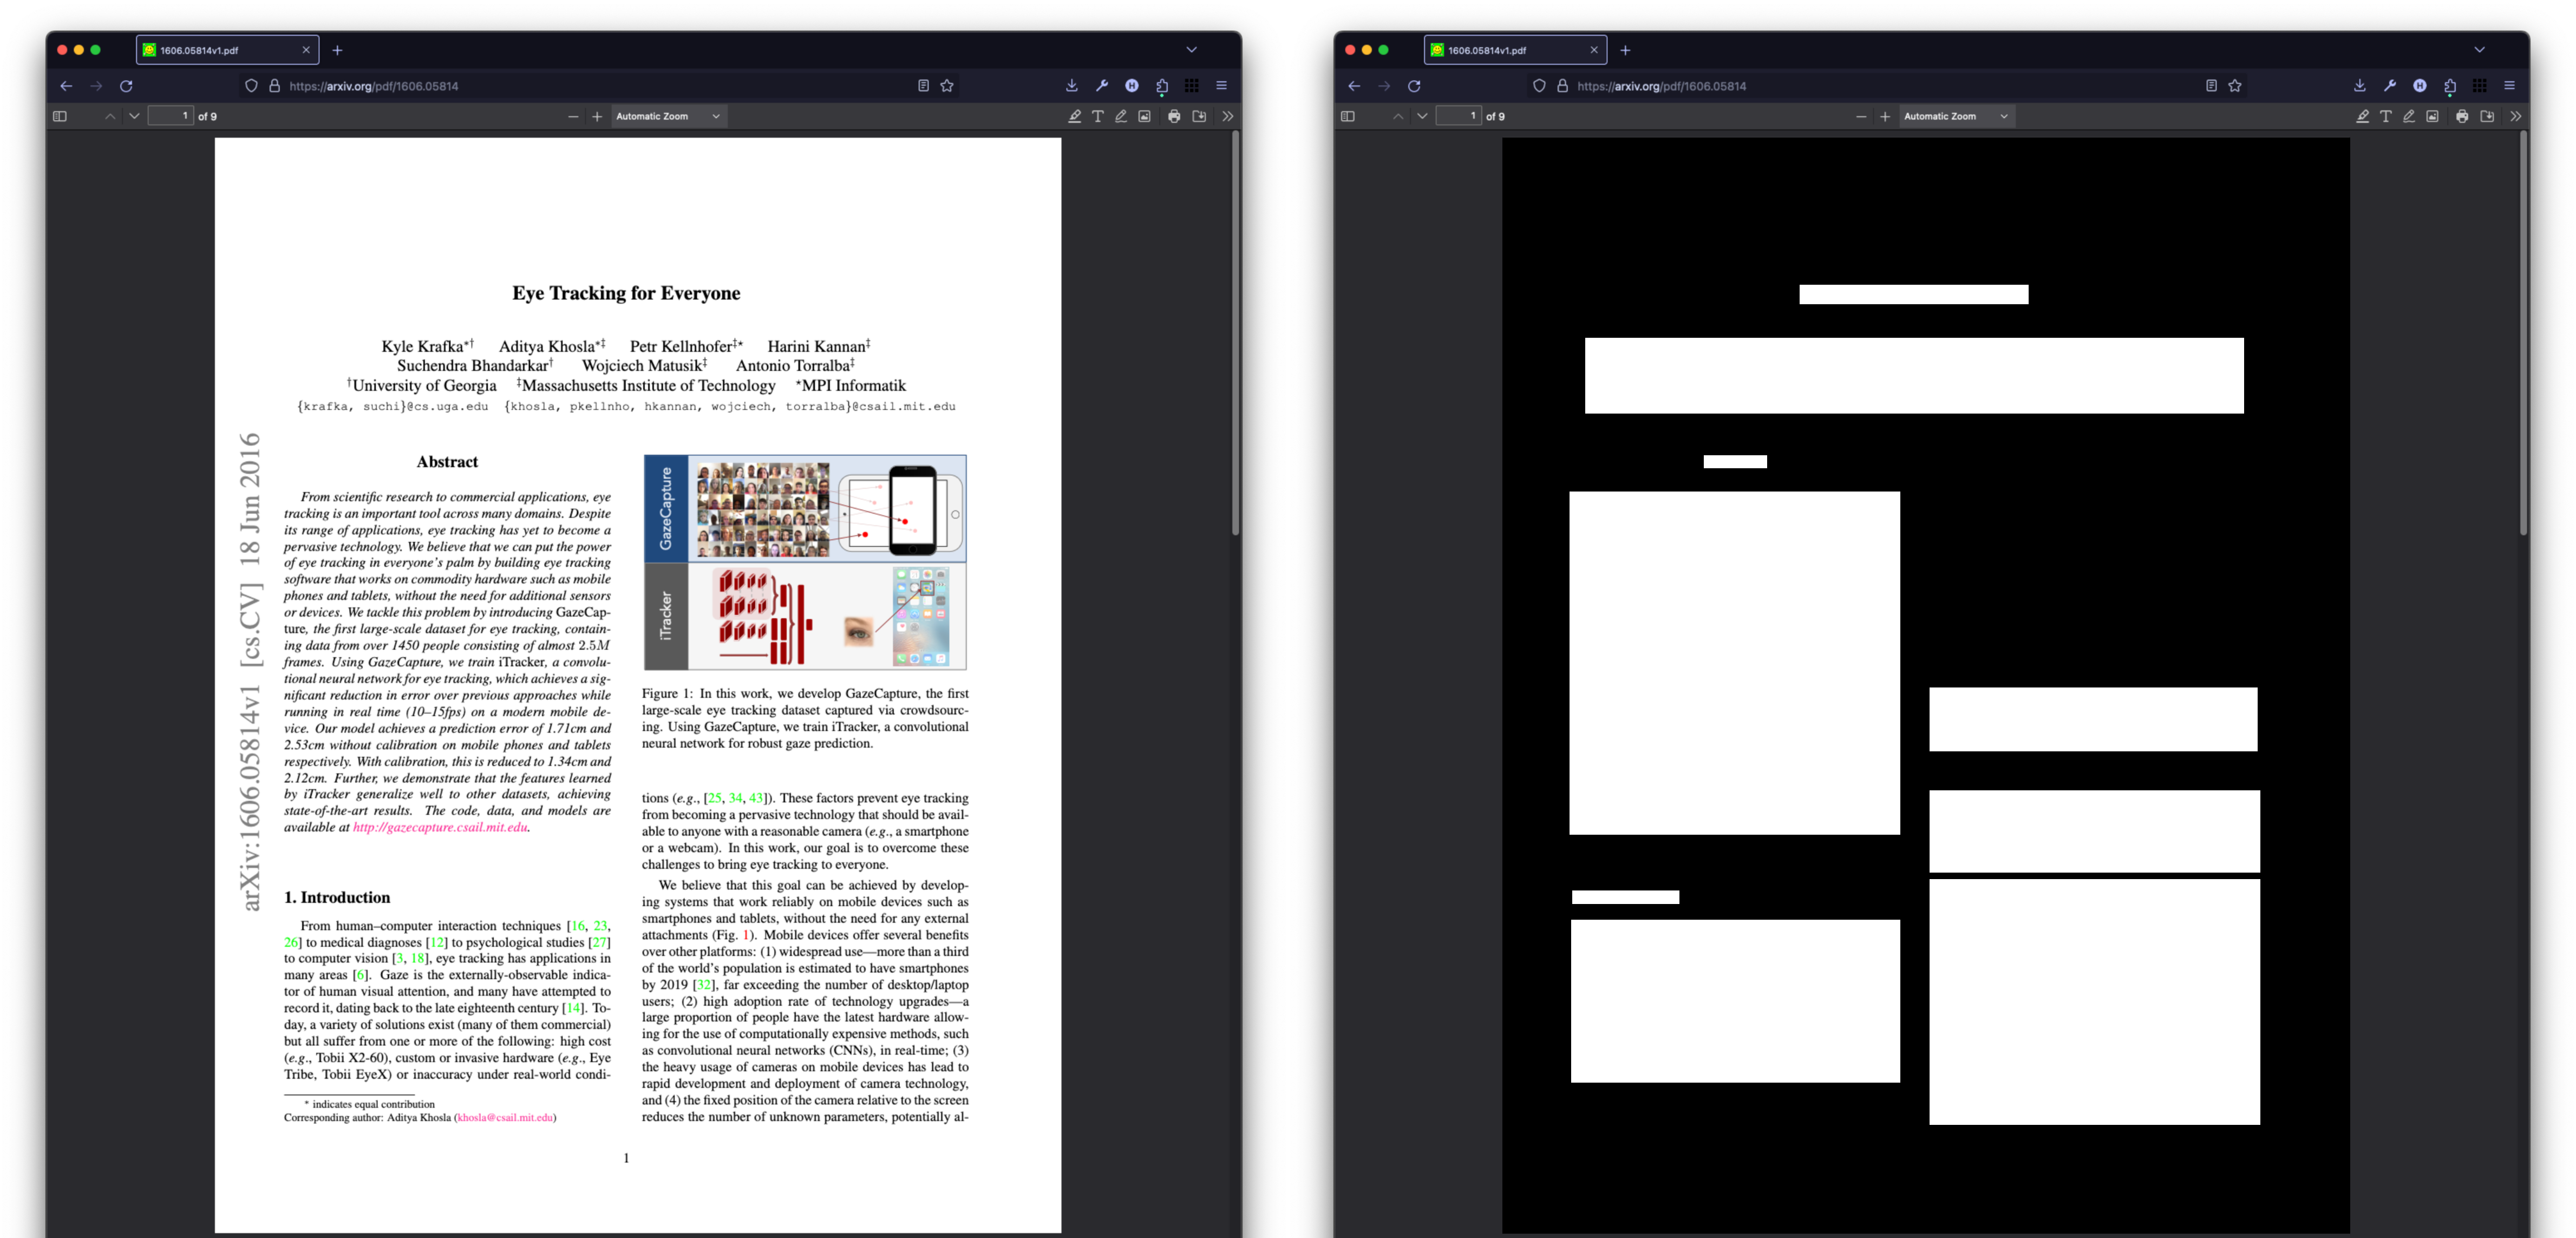
\includegraphics[scale=0.1]{../assets/binary-mask.png}
    \caption{An example of how a binary mask might look in a browser extension with a computer vision system to detect paragraphs}
\end{figure}

\section{User Interface} 

Browser extensions typically have a small ``pop-up'' window that appears in the upper right-hand of the browser when the extension icon is clicked. This is where the user can interact with the browser extension, for example, to check whether it is running or to configure its settings. To make sure that the browser extension is easy to use, the user interface of this popup window should be simple, and not confuse less technically-minded users. My design should look as close as possible to the mock-up as seen in~\autoref{fig:focusflow-mockup}. This design informs the user if the extension is currently active, and if it is not, it should display a warning message. 

\begin{figure}
    \begin{center}
        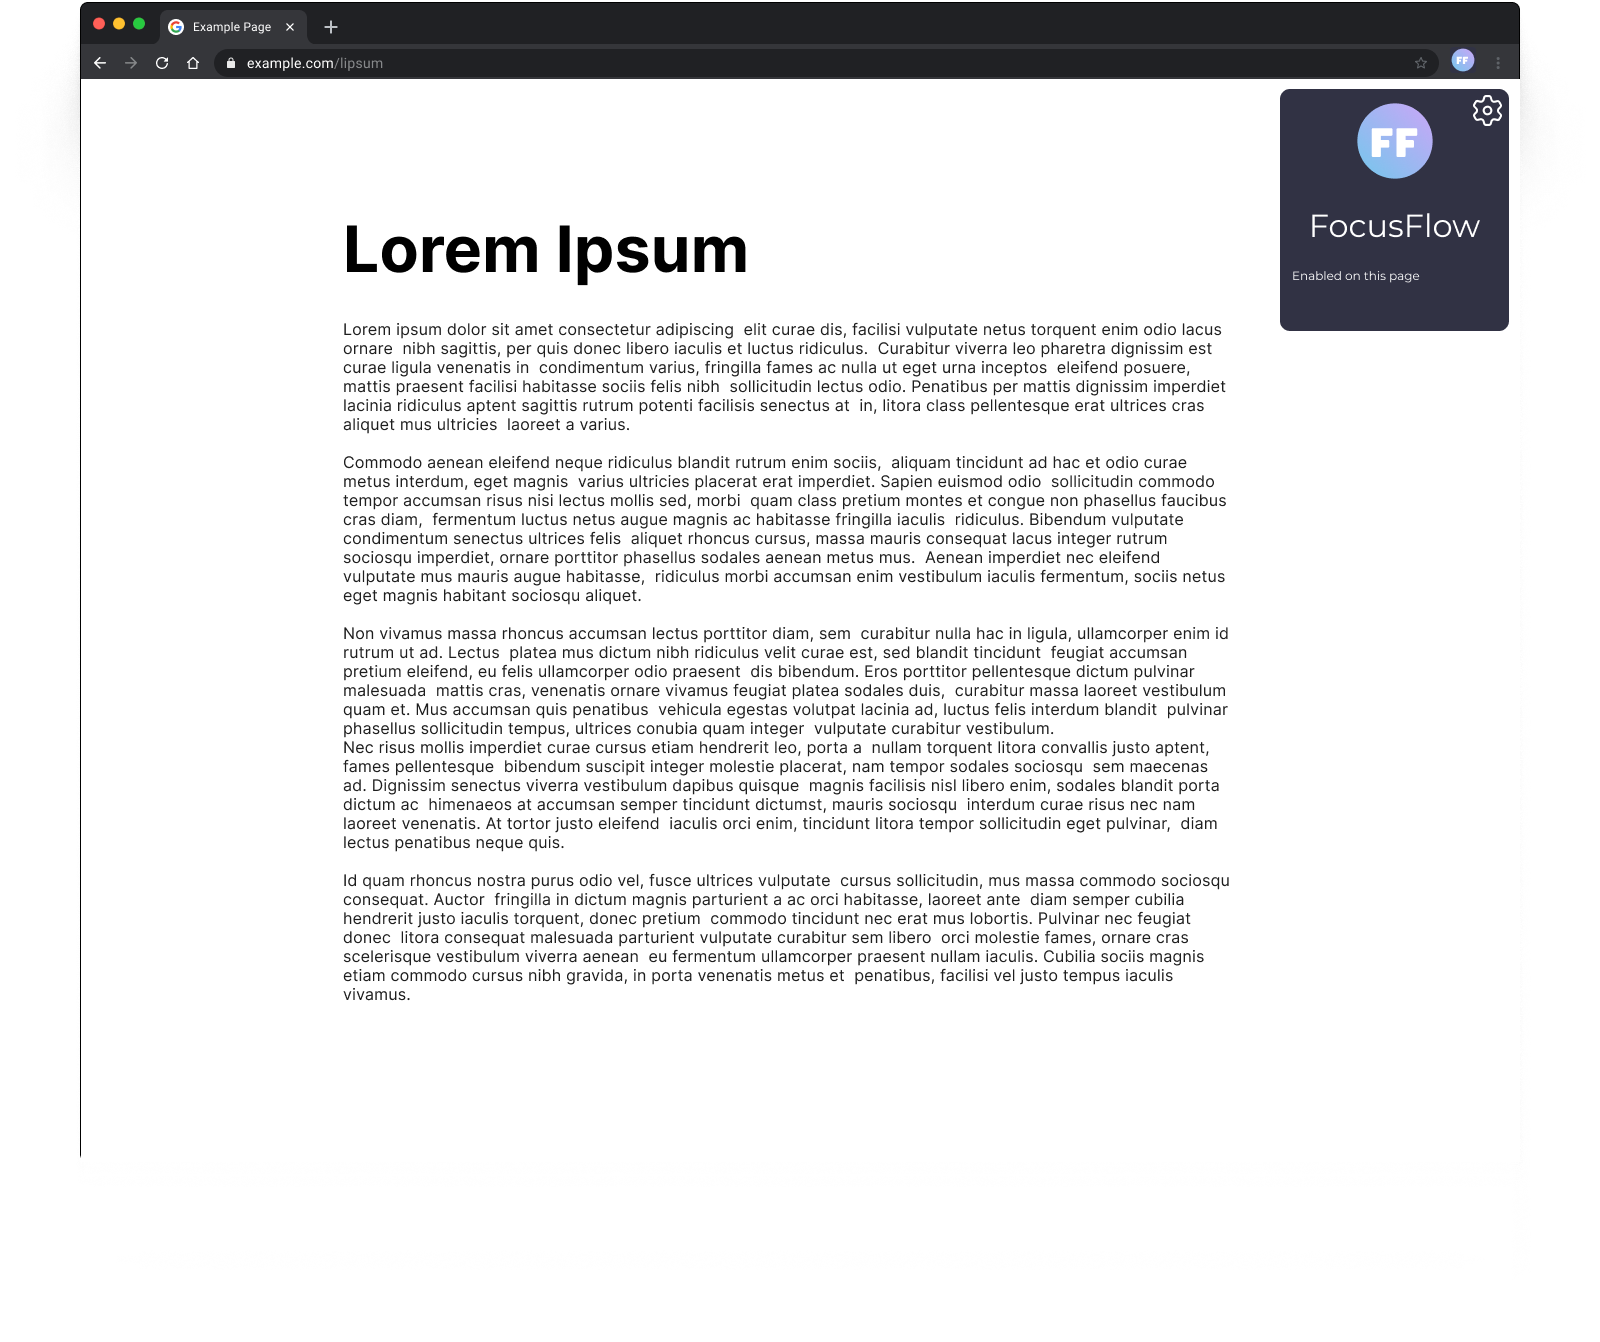
\includegraphics[scale=0.25]{../assets/user-interface-design.png}
    \end{center}
    \caption{Mockup for the FocusFlow browser extension}
    \label{fig:focusflow-mockup}
\end{figure}

When the user clicks on the cog icon in the top left of the extension pop-up, they will be taken to a page where they can configure the settings of the application. This page will allow the user to modify how the extension highlights the paragraph. See~\autoref{fig:ff-settings}. I considered adding a blacklist option to prevent the extension from running on certain pages. However, by denying the extension access to the camera, the web browser prevents the extension from running correctly, and no user information is captured. 

\begin{figure}
    \centering
    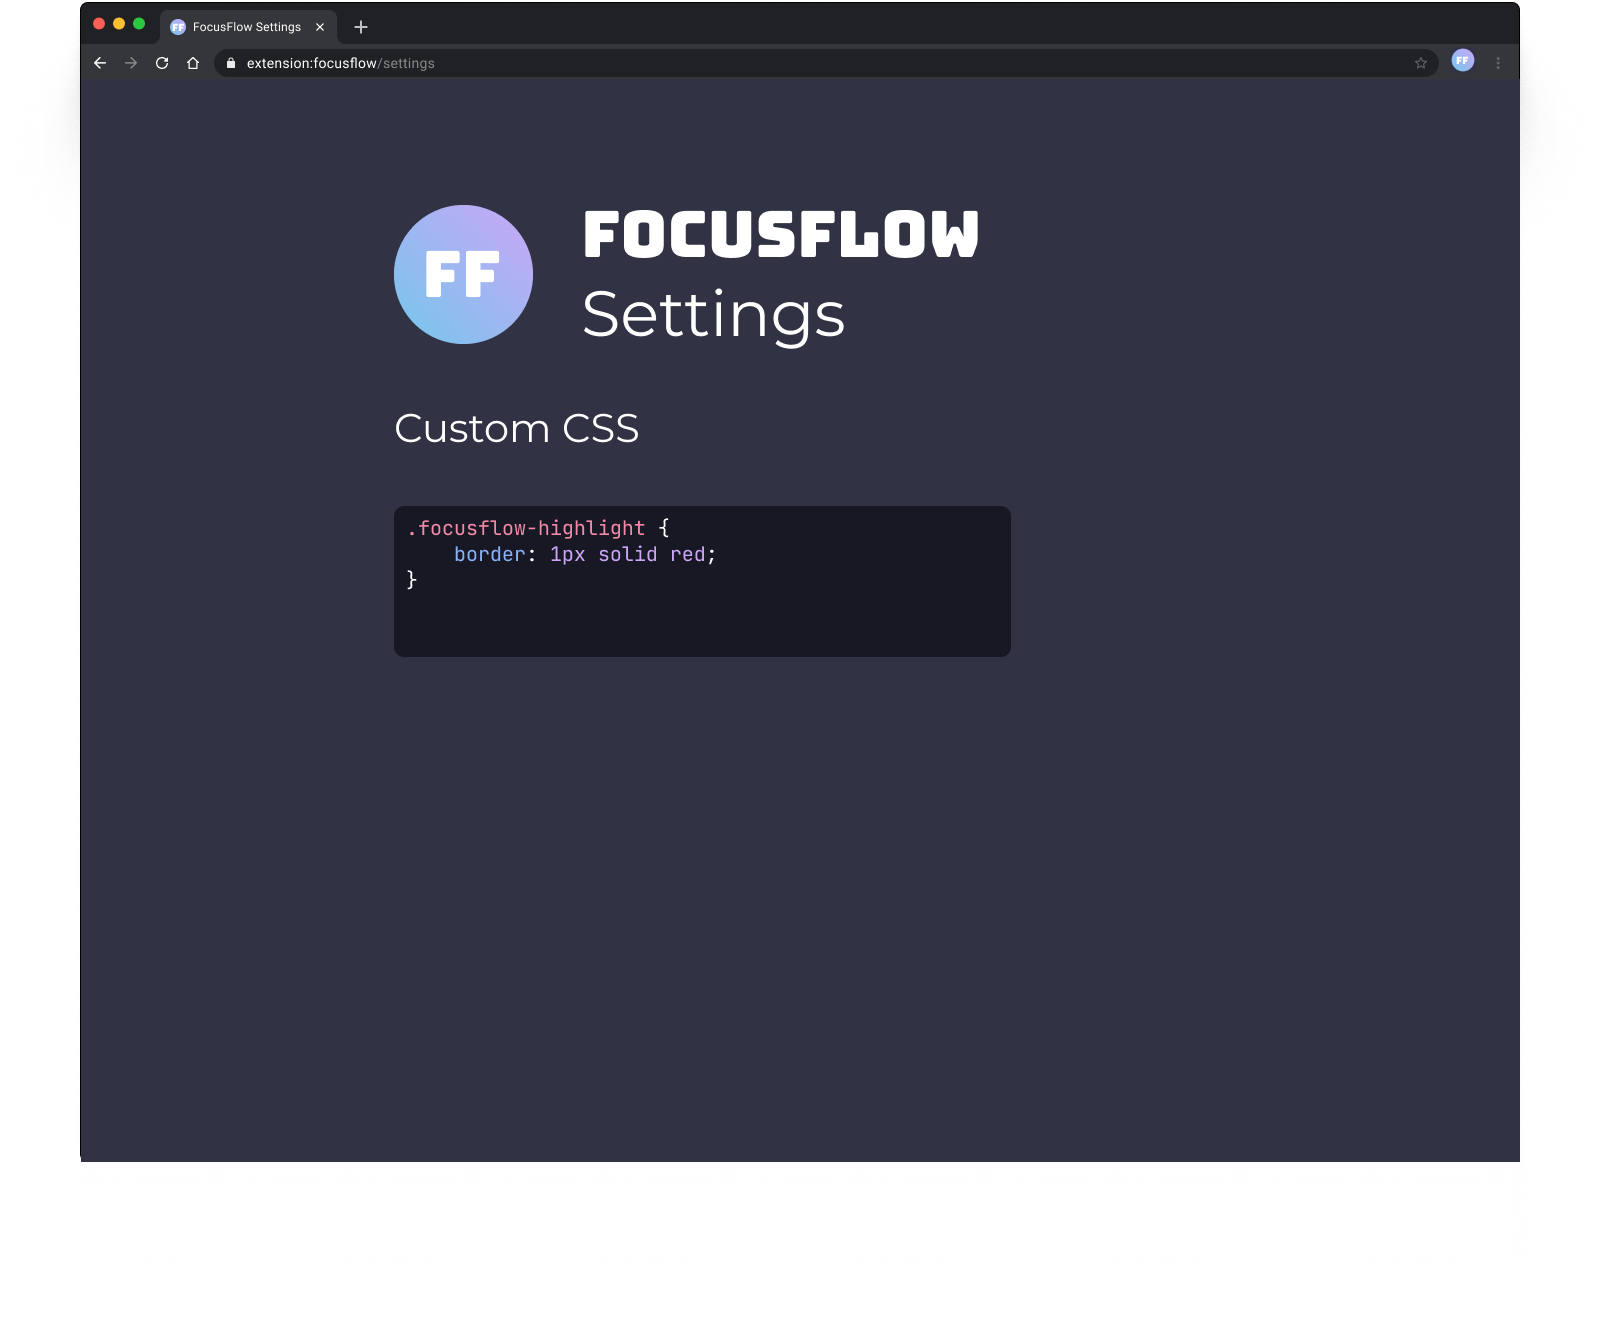
\includegraphics[scale=0.25]{../assets/focusflow-settings-page.png}
    \caption{The settings page for the FocusFlow Browser Extension}
    \label{fig:ff-settings}
\end{figure}

\section{Architecture}

My project will be comprised of two components: the browser extension which captures images of the user and generates a list of bounding boxes representing potential paragraphs being read, and an API which will host the gaze mapping model.

As explored in \autoref{ssec:ai-in-the-browser}, it is possible to perform inferences in the browser. However, there are trade-offs for this, such as having to transmit the trained machine learning model to every user, which can be very large. For example, the iTracker model trained on the MPIIFaceGaze dataset is approximately 25MB in size. For comparison, the median size of a desktop website in 2024 is 2.2MB~\cite{httparchive2024pageweight}. Having to load that large of a file would likely take a very long time for users with a slow internet connection and would negatively affect their experience. Furthermore, performing inference from a deep-learning model is very computationally expensive, and users with weak hardware could find their browser would slow down significantly when they try to perform the inference. 

For these reasons, I opted to remotely host the machine learning model, and communicate with it over a RESTful API~\cite{fielding2000phd}. This allows me to offload the computation of the inference to a dedicated application instead of running it through the browser. Running it natively allows the machine-learning model to make use of various hardware optimizations that the browser cannot access, such as NVidia's CUDA platform and Apple's MPS system. Furthermore, in a real-world deployment, I could host the API on a cloud platform such as AWS, and having the API ready to go would make this process far easier. 



The browser extension it




\chapter{FocusFlow Browser Extension}
\label{chap:methods}

% How the model was trained
% How the browser extension works
% How the extension communicates with the model
% How the model works
% Datasets

\section{Development of the FocusFlow Browser Extension}

I originally believed that developing an extension for Manifest V3 would significantly increase the complexity of development for my project. However, opting to use Manifest V2 would limit the potential user base of the system to Firefox users, which only make up approximately 3\% global browser traffic~\cite{statcounter2024browser}. I considered which would be the best approach to take, and eventually decided on developing my extension for the manifest V3 API, as it would allow virtually every web browser in the world to run the extension easily. As discussed in~\autoref{sec:browser-extension-background}, the manifest V3 API forbids browser extensions from loading and executing remote code, but still allows it to communicate with an API. This means that my extension is not effected by the new manifest API, and would be valid in both manifest versions 2 and 3. 

As part of my research, I discovered the Plasmo framework~\cite{plasmo}. This enables developers to rapidly develop cross-platform browser extensions. It handles all of the configuration and intricacies of developing browser extensions. I also found that when developing the extension, I was not hindered by any of the restrictions put in place by the Manifest V3 API. I chose to use it for my extension as it made the development process far more simple and provided a jumping-off point for development. It adds several elements such as background service workers, which run in the background of the browser and perform all of the processing necessary to implement my project. It also allows graphical elements of the browser extension such as the pop-up window, and the configuration page to be defined using modern, front-end tooling, such as React, Vue and Svelte using a superset of JavaScript called typescript which provides typing to the language. This makes development far easier, and more maintainable.

The browser extension is activated on page load. Once the extension is loaded into the context of the webpage, it requests access to the user's webcam using the Media Capture and Streams API, which is a part of all major browsers and allows for the manipulation of audio and video streams. If the user does not allow access to the webcam, the extension will not function. It then gets a list of all elements within the current viewport. The viewport is a concept which represents the visible area of a page. This list is then filtered based on the tag name, elements that contain text are kept, and others such as \texttt{<div>}, \texttt{<img>}, and \texttt{<section>} are discarded. This is necessary as many HTML elements contain no text, while still being visible on the page. 

The browser then waits until the page it's running on goes out of focus, meaning the user has switched browser tabs, and takes an image capture from the webcam. It detects this using the JavaScript Page Visibility API~\cite{pagevisibility}, which fires an event when the page goes in or out of focus. It passes that image, and information about what kind of device the browser extension is running on, i.e.\ desktop or mobile device, to a local python API over the Hyper-Text Transfer Protocol. The python API then performs inference on that image and passes the gaze location back to the browser extension, which then determines which element the gaze location intersects with, and highlights it. See Fig~\ref{fig:flowchart} for a graphical explaination as to how the extension functions. 

\begin{figure}
    \begin{center}
        
\includegraphics[scale=0.25]{../assets/flowchart.png}
    \end{center}
    \caption{The flowchart outlining the functionality of the browser extension}
    \label{fig:flowchart}
\end{figure}

\section{Python Server}

I developed the Python server using FastAPI, a library built on top of Flask which allows rapid development of REST APIs. I chose to use FastAPI as I am already familiar with the framework due to the ease of use, and excellent performance~\cite{klenov2015benchmark}. Other, more performant frameworks exist for this use case such as BlackSheep~\cite{prevato2018blacksheep}, but I am unfamiliar with them, and they don't have as much community support behind them.  

The API only has two endpoints, one to verify that the server is running, and another to perform inference on an image. The image is encoded in the form data, meaning it is encrypted while in transit. It also takes a parameter telling the API which model to perform the inference on, the model trained on gazecapture for mobile devices, and the model trained on MPII face gaze for desktop devices. 

As the API runs locally on the user's device, there is no need for the content of the request to be encrypted. However, in a real-world deployment of this project where the API is hosted on a remote server, an SSL certificate should be obtained for the API to ensure malicious actors cannot intercept the images taken from the browser extension while the data is in transit between the browser extension and the API. 


\section{Model Selection}

When considering models, I wanted something that does not rely on any other systems, such as head pose detection, as adding additional inference would amplify errors between models and would make the predictions less accurate. For this reason, I opted to use an appearance-based model which predicts a 2D point of gaze. For this reason, I chose to use the iTracker model as outlined in~\cite{krafka2016eye}. This model has shown promising performance in both a desktop and mobile context, \(7.67\text{cm}\) for desktop applications, \(2.81\text{cm}\), \(1.86\text{cm}\) in tablet and phone environments respectively~\cite{cheng2021survey}.

\section{Datasets}

To develop the deep learning model, I used both the Gazecapture and MPIIFaceGaze datasets. 

\subsection{MPIIFaceGaze}\label{ssec:mpii-face-gaze}

I trained a model on the MPII Face Gaze dataset~\cite{zhang2019mpii}. This dataset was captured from a smaller pool of participants (15) and considers gaze mapping within the context of devices such as laptops. The goals of this dataset were to capture images of participants outside of laboratory conditions and to record images of participants over a longer period. To achieve these goals, researchers opted to capture the data on participants' devices, as they typically are only operated by a single user throughout the day for a long period. As laptops can be used anywhere, the dataset exhibits wide variation in lighting conditions, and head pose from participants using their devices in a variety of environments. 

The dataset was collected using a background service running on their laptop. Every 10 minutes, the service would ask users to fixate on a random series of 20 on-screen positions. The ground truth data were collected using the moving dot stimulus as outlined in~\cite{kassner2014pupil}. The dots would slowly become more transparent. Once the dot was about to become fully transparent, the user was instructed to press the space bar to ensure their attention was focused on the dot. This method collected a total of 213,659 images from 15 participants. 

The diversity of participants in comparison to Gazecapture is significantly worse. Out of the 15 participants, only six were female, and a majority were White or Asian. Gazecapture has a far better range of diversity among its participants due to its crowdsourced nature, however, there are no available statistics as to the ethnic makeup of the participants in the dataset. Despite this, I chose to use this dataset to train the iTracker model for the desktop model for several reasons, including the fact that the repository~\cite{krafka2016eye,cheng2021survey} includes methods to process and load the dataset into the model, and the annotations include the 2D point of gaze and information about the size of the screen. 

\subsubsection{Data Augmentation}

The MPIIFaceGaze dataset does not contain any subsets for testing and validation, so I had to create them myself. I decided on a 66.6/20/13.3\% split for training, validation, and testing. This split was performed on each participant to ensure the model didn't see any images of the participants within the training set. Members of each subset of the dataset were randomly selected. 

I also had to modify the ground truth data. I wanted the trained model to work on screens of any size, while the training data included a data point of the screen size in pixels divided by the screen size in millimeters, which was then divided by 100 and fed into the model, the web browser does not expose any behaviour to easily find the size of the screen in millimeters and thus made it difficult to get the true gaze location. I changed this ratio to the screen size in pixels, and then multiplied the gaze location, measured in pixels from the origin by the reciprocal of the screen size. This restricts the range of values the true gaze location can take to 0-1 and allows the model to learn the 2D gaze position for any screen size. 

After augmentation, some of the true gaze locations ended up lying outside of the screen. To remedy this, I clamped the ground truth data between 0 - 1 before feeding it into the model. This prevents the model from predicting gaze locations that lie outside of the screen, and in the worst case will end up opting for the bottom right of the screen. 

\subsection{Gazecapture}\label{sec:gazecapture}

The Gazecapture dataset was collected through crowdsourcing. This allowed the authors to get a very high number of subjects ($1474$), and therefore a high number of images in the dataset ($2,445,504$). Participants were gathered using Amazon's Mechanical Turk service~\cite{mturk} and asked to download a free app on their device. The Mechanical Turk platform allows researchers and developers access to a large, diverse on-demand workforce. Once opened, the app asked the participants to enable airplane mode to avoid distractions while collecting the data. The app then displays a pulsating red dot on the screen for approximately 2 seconds~\cite{krafka2016eye}, and the camera begins recording 0.5 seconds after the dot is displayed, once the recording is complete, the dot disappears. The app then displays \textit{L} or \textit{R} on the screen for a short window of time, 0.05 seconds. The user must press either the left or right side of the screen depending on what label was displayed to measure their engagement with the application. If they get it wrong, they are warned and required to repeat the previous dot. The app also makes use of the real-time face detector built into iOS to ensure their face is visible in the video captures.

By making use of crowdsourcing to create datasets, the diversity of participants is significantly greater than researchers would otherwise get. Gazecapture has a wide variety of ethnicities, lighting conditions, head poses, appearances, and backgrounds among the participants.

During the collection of the data, participants were asked to move their devices around and to look at their screens from a variety of positions. This means that the dataset exhibits a wide variety in the head pose, and gaze directions when compared to other comparable datasets, such as TabletGaze~\cite{huang2016tabletgaze} and MPIIGaze~\cite{zhang15cvpr} with the intention that the model can better generalize the location of gaze under a variety of conditions.


\section{Training}
\label{sec:training}

The training was performed on a single Mac Studio with an M1 Ultra Chip, clocked at 3.2GHz, with a 24-core GPU, 16-core ``Neural Engine'' and 64GB of memory. Apple's recent developments into their own, custom CPUs such as the M1 have included cores dedicated to the training and use of neural networks, known as their neural engine. Making use of this specialized hardware enables faster training of machine learning models when compared to using the CPU, similar to Nvidia's CUDA platform. 

When training with MPIIFaceGaze, it took approximately 30 hours to perform 25 epochs, with a learning rate of 0.001. As we see in Fig.~\ref{fig:val}, the validation distance decreased practically every epoch, but not by very much. It used Mean-Squared Error as the loss function, and the validation dataset had two participants within it. The validation error began to plateau around 0.38 after a few epochs of training, as is similar to the training loss (\autoref{fig:loss}). The training loss began around 0.35, and rapidly converged around 0.08. This indicates that improvements from further training would likely be marginal, and to better estimate the location of gaze, a larger dataset, hyperparameter optimisation, or a different architecture entirely may be necessary. I believe that the best option to improve performance would be to use a larger dataset, as the MPIIFaceGaze dataset is very small in comparison to other larger datasets. 

\begin{figure}
    \begin{center}
        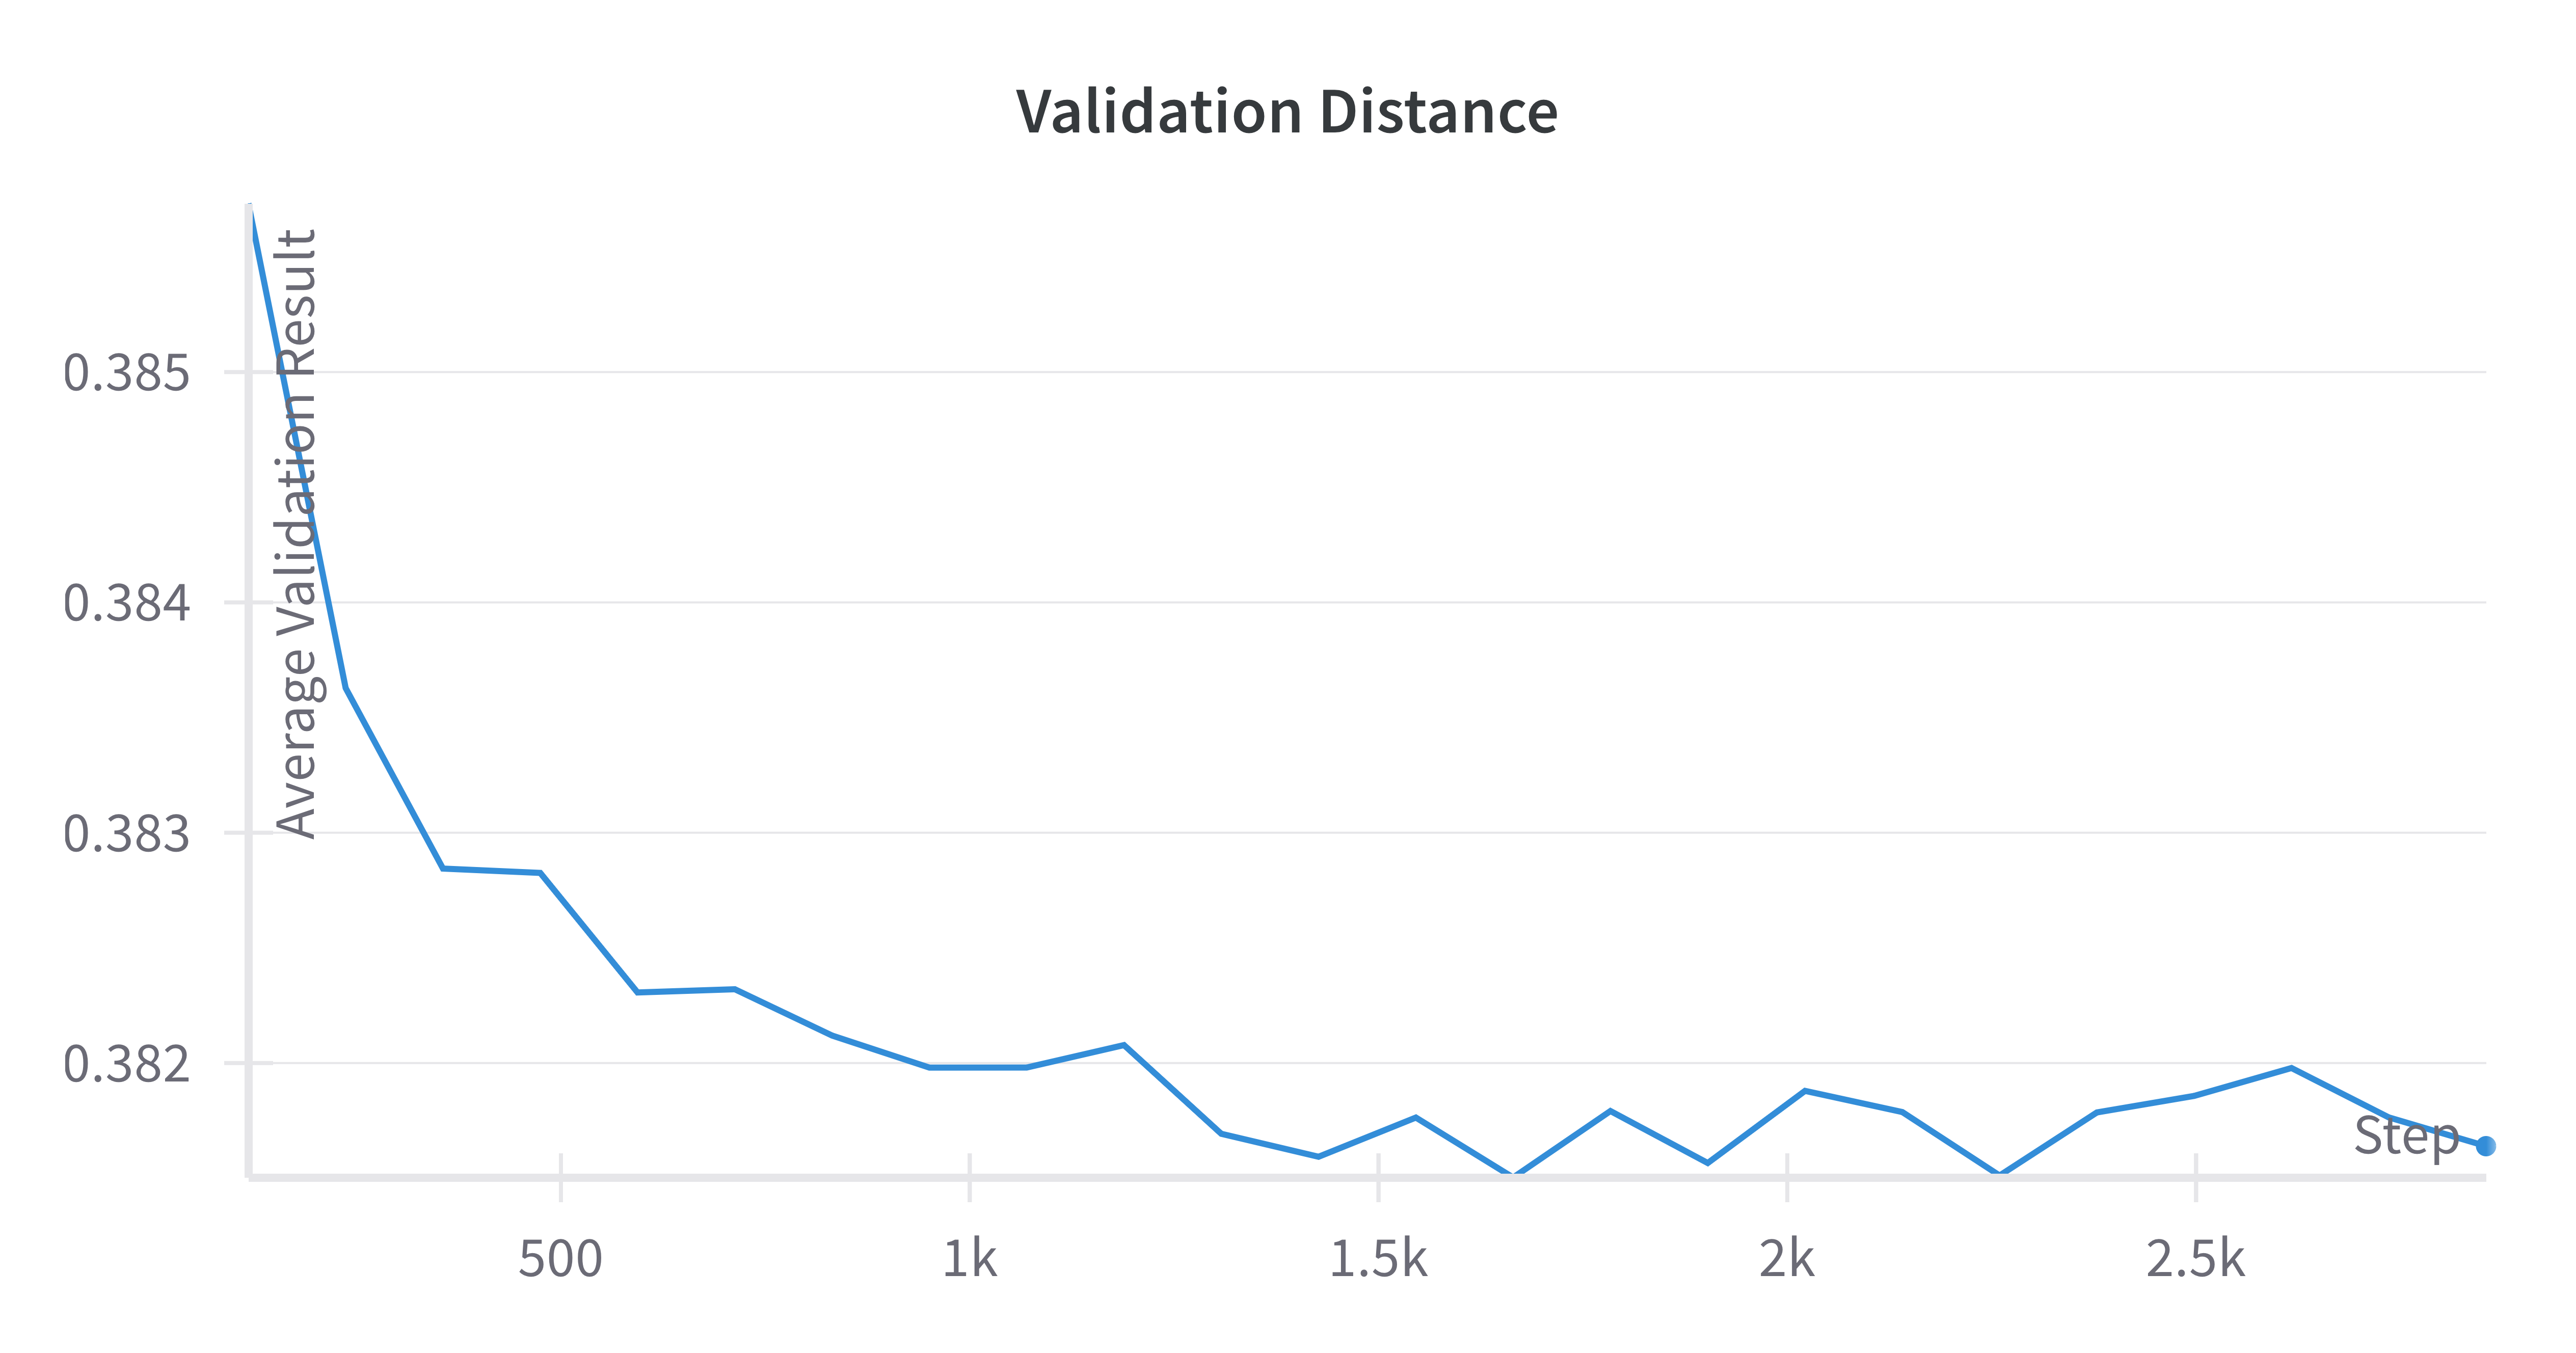
\includegraphics[scale=0.1]{../assets/Validation Distance.png}
    \end{center}
    \caption{The average validation error of iTracker with MPII Face Gaze}
    \label{fig:loss}
\end{figure}

\begin{figure}
    \begin{center}
        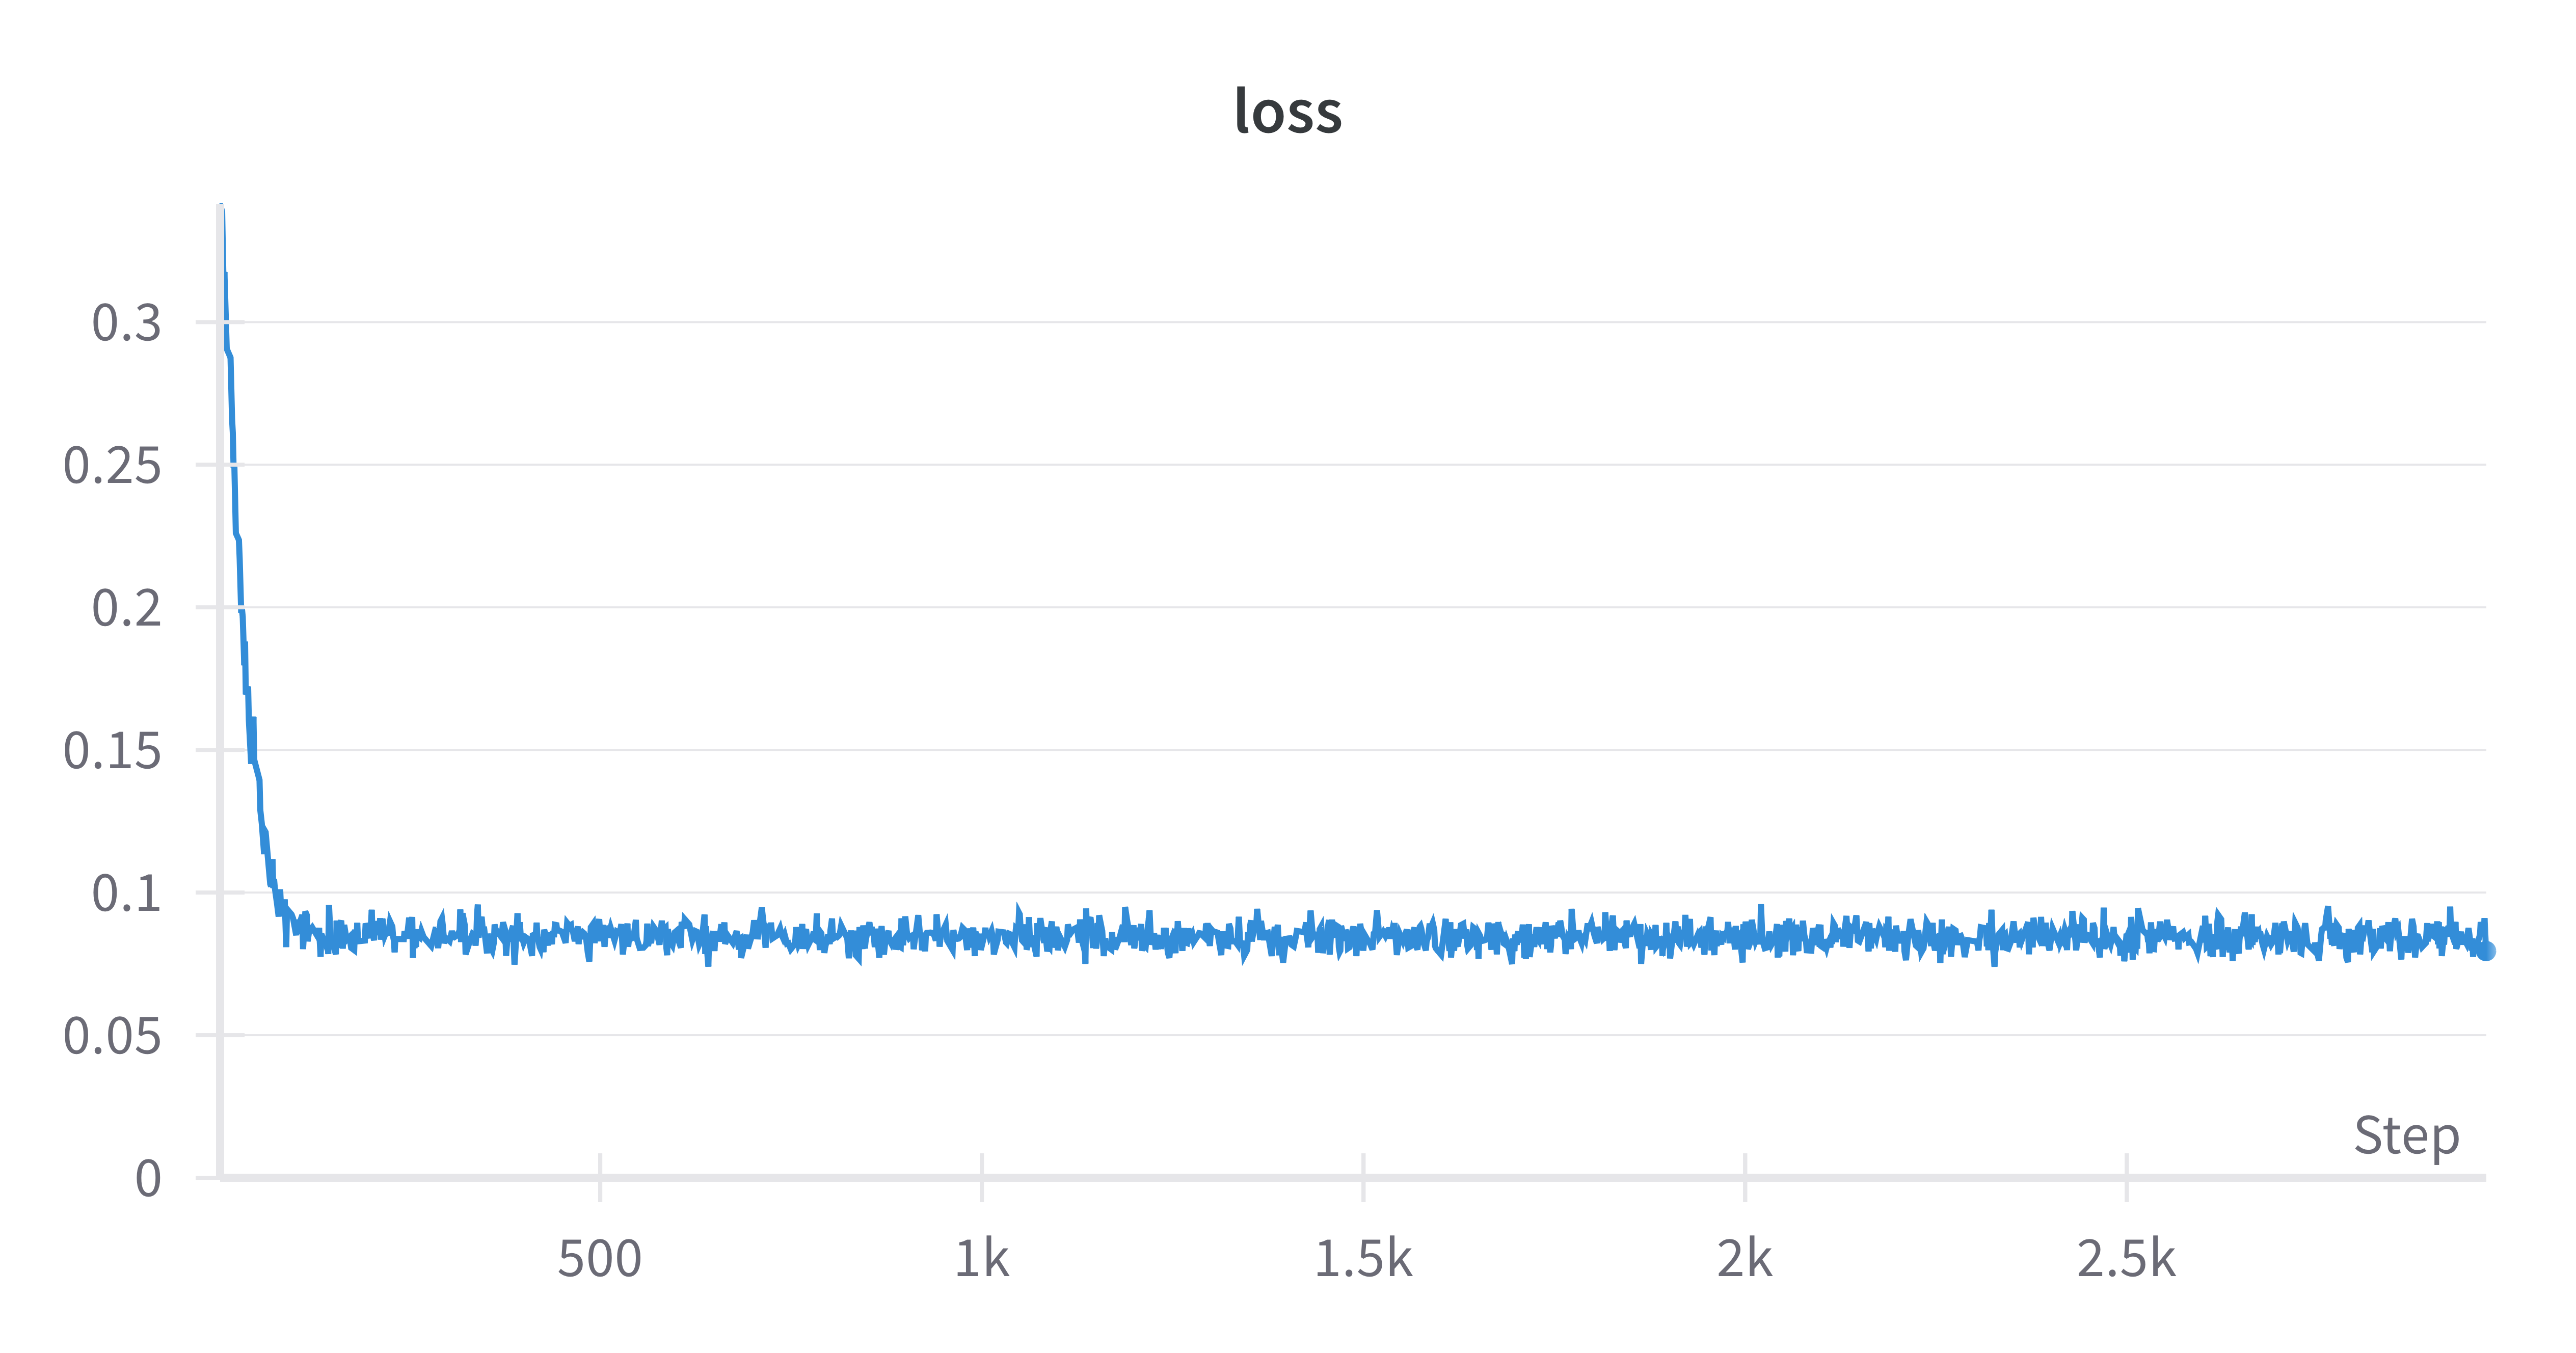
\includegraphics[scale=0.1]{../assets/Training Loss.png}
    \end{center}
    \caption{The training loss of the iTracker model with MPII Face Gaze}
    \label{fig:val}
\end{figure}


\chapter{Evaluation of the FocusFlow Browser Extension}
\label{chap:results}

This chapter will evaluate the effectiveness of the browser extension I developed. It will cover how well the final product meets the requirements outlined in ~\autoref{sec:requirement-analysis}, how effective the machine learning model I developed is, and under what conditions the performance of the extension is optimal. I will discuss the effectiveness of the machine learning model in \autoref{sec:itracker-eval}, and how well the final product meets the requirements in ~\autoref{sec:post-devel-requirement-analysis}.

\section{Evaluation of the Machine Learning Model}\label{sec:itracker-eval}

This section will evaluate the performance of my deep-learning model which underpins the browser extension. I will discuss its performance in predicting gaze locations and how it relates to the browser extension I developed, how effectively it performs under different conditions, and overall whether the model is suitable for the automatic bookmarking system I designed.

As explored in Section~\ref{sec:training}, the machine learning model achieved a normalised test error of approximately 0.38. This correlates to approximately 10cm horizontal error and 7.5cm vertical error, on the assumption that the device it is running on has a screen that is approximately 30cm by 20cm. This is not ideal however I found that when running my extension in the real world, it could detect the correct paragraph in most cases. It would sometimes detect the incorrect paragraph, by either selecting the paragraph directly above or below the location of true gaze. This indicates that most of the error originates from the vertical component of the gaze location. This could be explained by the fact that when interacting with a web page, users will typically scroll such that the paragraph they are currently reading is at the top of the page. To test this, I tried using the extension and focussing on a paragraph in the middle of a screen. When I did this, I found that the browser extension would opt to highlight paragraphs above or below the location of the paragraph I was focussing on. This indicates that the vertical component of the predicted gaze location is not nearly accurate enough. 

Furthermore, the horizontal component of gaze is often weighted as less important than the vertical component. This is because, on web pages, paragraphs are typically aligned in a single-column arrangement, meaning each paragraph is directly on top of one another, perhaps with some vertical padding for aesthetic or readability reasons. On a hypothetical two-column website, I presume that the model would have similar problems predicting the paragraph on the left or right side of the screen. However, I was unable to test this as most websites do not opt for a two-column layout, instead opting for a single column with a shorter line length to improve readability. 

I was also unable to train the iTracker model on the gazecapture dataset. This is because the gazecapture dataset is very large when compared to the mpii face gaze dataset. For example, it has a total of approximately 1500 participants for a total of approximately 2.5 Million images, whereas MPII Face Gaze has a total of 15 participants for a total of 40,000 images. While this would mean that the model is better trained in performing gaze inference, it would've also taken significantly longer to train and optimize, the estimation for training time provided by the authors of the ``Eye tracking for everyone'' paper~\cite{krafka2016eye} was nearly a month. This is why I considered performing transfer learning to improve the time required to train the model. However, due to time constraints, I was unable to perform this fine-tuning of the model.

To test how the model performs under a variety of lighting conditions, I have designed an experiment that will take a single image from the in-built camera, and perform gamma correction, which effectively darkens an image. This emulates different lighting conditions the browser extension may be used in while keeping the head and screen pose of the user the same. The results for this experiment are demonstrated in \autoref{fig:lighting}. This shows that under different lighting conditions, the model predicts gaze at similar locations. However, when the lighting conditions get sufficiently dark, i.e. a $\gamma$ value of less than 0.4, the face detection model used for pre-processing fails to find the face within the image. This shows that the machine learning model is robust to changes in the lighting conditions of the image. 

I also generated a heatmap that shows where the machine learning model is most likely to predict the location of the gaze of a user to get an idea of how much variation there is in its responses. This process involved capturing a large number of samples, then plotting them on a grid where their colour is the relative frequency of that location. This should indicate if the model has a bias towards a certain location and if any modifications to the model are required. In total, I captured $6924$ samples, and the results are in~\autoref{fig:heatmap}. We see that the model typically predicts gaze around $(0.5, 0.5)$. As the MPIIFaceGaze dataset which this model was trained on randomly selects locations on the screen, we can assume that there is a relatively even split between gaze locations on the top, bottom, left and right of the screen. Thus, predictions typically occurring around the center of the screen are to be expected, and also indicate the model underfitting. This could be remedied using a larger dataset. We also see a strong linear correlation between the $x$ and $y$ coordinates of the screen. This further supports my hypothesis of the model underfitting the training dataset. I believe this is due to the MPIIFaceGaze model not including enough variety of gaze locations in its annotations. See~\autoref{fig:log-mpii} for a plot of locations annotations found within the MPIIFaceGaze dataset.

\begin{figure}
    \centering
    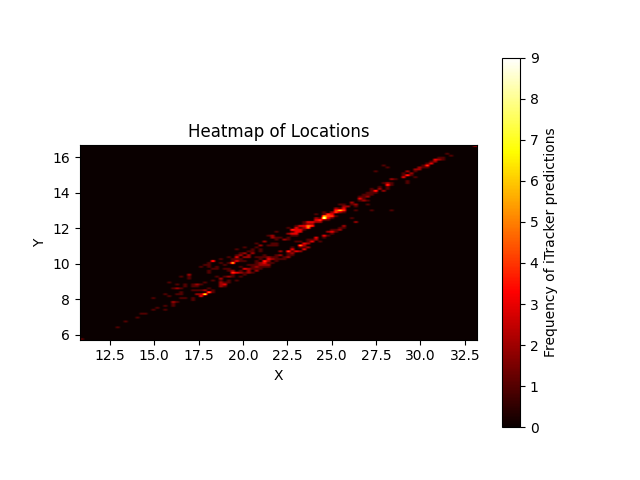
\includegraphics[scale=1]{../assets/heatmap.png}
    \caption{Heatmap of Gaze Locations made by iTracker}
    \label{fig:heatmap}
\end{figure}

\begin{figure}
    \begin{center}
        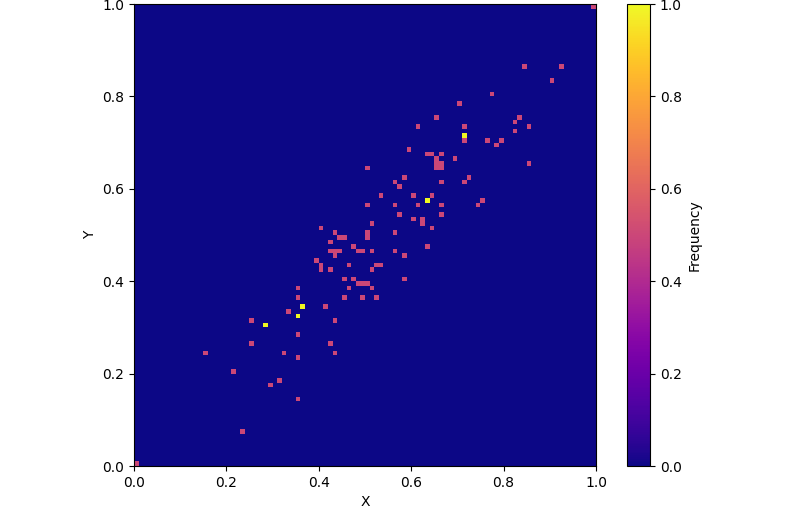
\includegraphics[scale=0.5]{../assets/log-mpii.png}   
    \end{center}
    \caption{Locations of gaze within the MPIIFaceGaze dataset}
    \label{fig:log-mpii}
\end{figure}


\section{Post-Development Requirement Analysis}
\label{sec:post-devel-requirement-analysis}

\begin{center}
\begin{tabularx}{\textwidth}{|X|c|c|c|X|}
    \caption{Analysis of Requirements Compliance Table} \\ 
    \hline
    \textbf{Requirement} & \textbf{Kind} & \textbf{Achieved} & \textbf{Evidence} & \textbf{Notes} \\ 
    \hline

    The browser extension must run on as many possible browsers as possible, including all of the most popular such as Chrome, Firefox, Edge, and UC browser. & Functional & Yes & \autoref{fig:browser-support} & I was unable to test UC browser as it is not supported on my laptop which runs on Mac OS, however, it is based on the blink browser which means it should be supported as all browsers tested with the exception of firefox are based on.  \\
    \hline
    The browser extension must request permission from the user to access their integrated camera. & Functional & Yes & \autoref{fig:ff-camera} & \\
    \hline
    The browser extension must highlight the paragraph that they were last reading before the page went out of focus.  & Functional & Partial & v & The accuracy of the machine learning model is relatively poor and it often gets the element wrong, but close to the true paragraph location \\
    \hline
    The browser extension must be able to determine the platform it's currently running on, i.e.~mobile, or desktop. & Functional & Yes & v & Assuming all mobile devices have an \texttt{innerWidth} of less than 1024 pixels. \\
    \hline
    The browser extension must securely transmit the images taken from the web page to the API & Functional & No & ~ & Images are not encrypted, but as the API runs locally, malicious agents are limited in their ability to intercept these images. However, in a real-world deployment, the data should be transmitted over HTTPS. \\
    \hline
    The machine learning model must predict the location of the user gaze within approximately \(2.5\text{cm}\) of the user's location gaze  & Functional & No & See notes & Model achieved a training error of approx 40\% which correlates to 10cm x 7.5cm assuming 30cm x 20cm screen size \\
    \hline
    The machine learning model must work in a variety of lighting conditions. & Functional & Yes & \autoref{fig:lighting} & As demonstrated in~\autoref{fig:lighting}, the model works well under a variety of lighting conditions. To test this, I took an image and performed gamma correction on it with a variety of $\gamma$ values. As seen in the results, the model predicts the gaze location at a similar location for each image, except when $\gamma$ falls below $0.4$, at which point the processing step fails, and is unable to detect a face within the image. \\ 
    \hline
    The machine learning model must work with a variety of head poses.  & Functional & Partial & ~ & \\
    \hline
    The machine learning model must work on devices with a variety of screen sizes  & Functional & Yes & ~ & The model predicts the gaze location in a normalised space, and is converted to reflect their gaze location on their screen  \\ 
    \hline
    The user must be able to configure how the browser extension highlights paragraph elements & Functional & No & ~ & I was unable to implement this due to time constraints \\
    \hline
    The machine learning model must not be biased, i.e.~it works only for caucasian users. & Non-Functional & ~ & ~ & \\ 
    \hline
    The web browser should work on both mobile and desktop browsers. & Functional & Partial & ~ & The browser extension loads on a mobile browser, but the backend API does not currently support mobile gaze inference as I was unable to perform transfer learning on the trained desktop model  \\  
    \hline
    The browser extension should display an error message on the page if the gaze estimation API is unavailable & Functional & No & & I was unable to implement this due to time constraints. \\ 
    \hline 
    The browser extension should display an error message on the page if the user denies access to their device's camera  & Functional & no & & I was unable to implement this due to time constraints. \\ 
    \hline 
    The browser extension should not run on blacklisted websites & Functional & Yes & & I didn't have to implement this as the browser has its functionality to request access to the camera. If they do not allow access, the extension does not add the event listeners which handle capturing images and performing gaze inference. The user has the option to remember this setting so the browser does not repeatedly ask for permission to use this API, which effectively acts as a blacklist of sites that it does not run on. \\ 
    \hline 
\end{tabularx}
\end{center}


\begin{figure}
    \centering
    \begin{subfigure}[b]{0.45\textwidth}
        \centering
        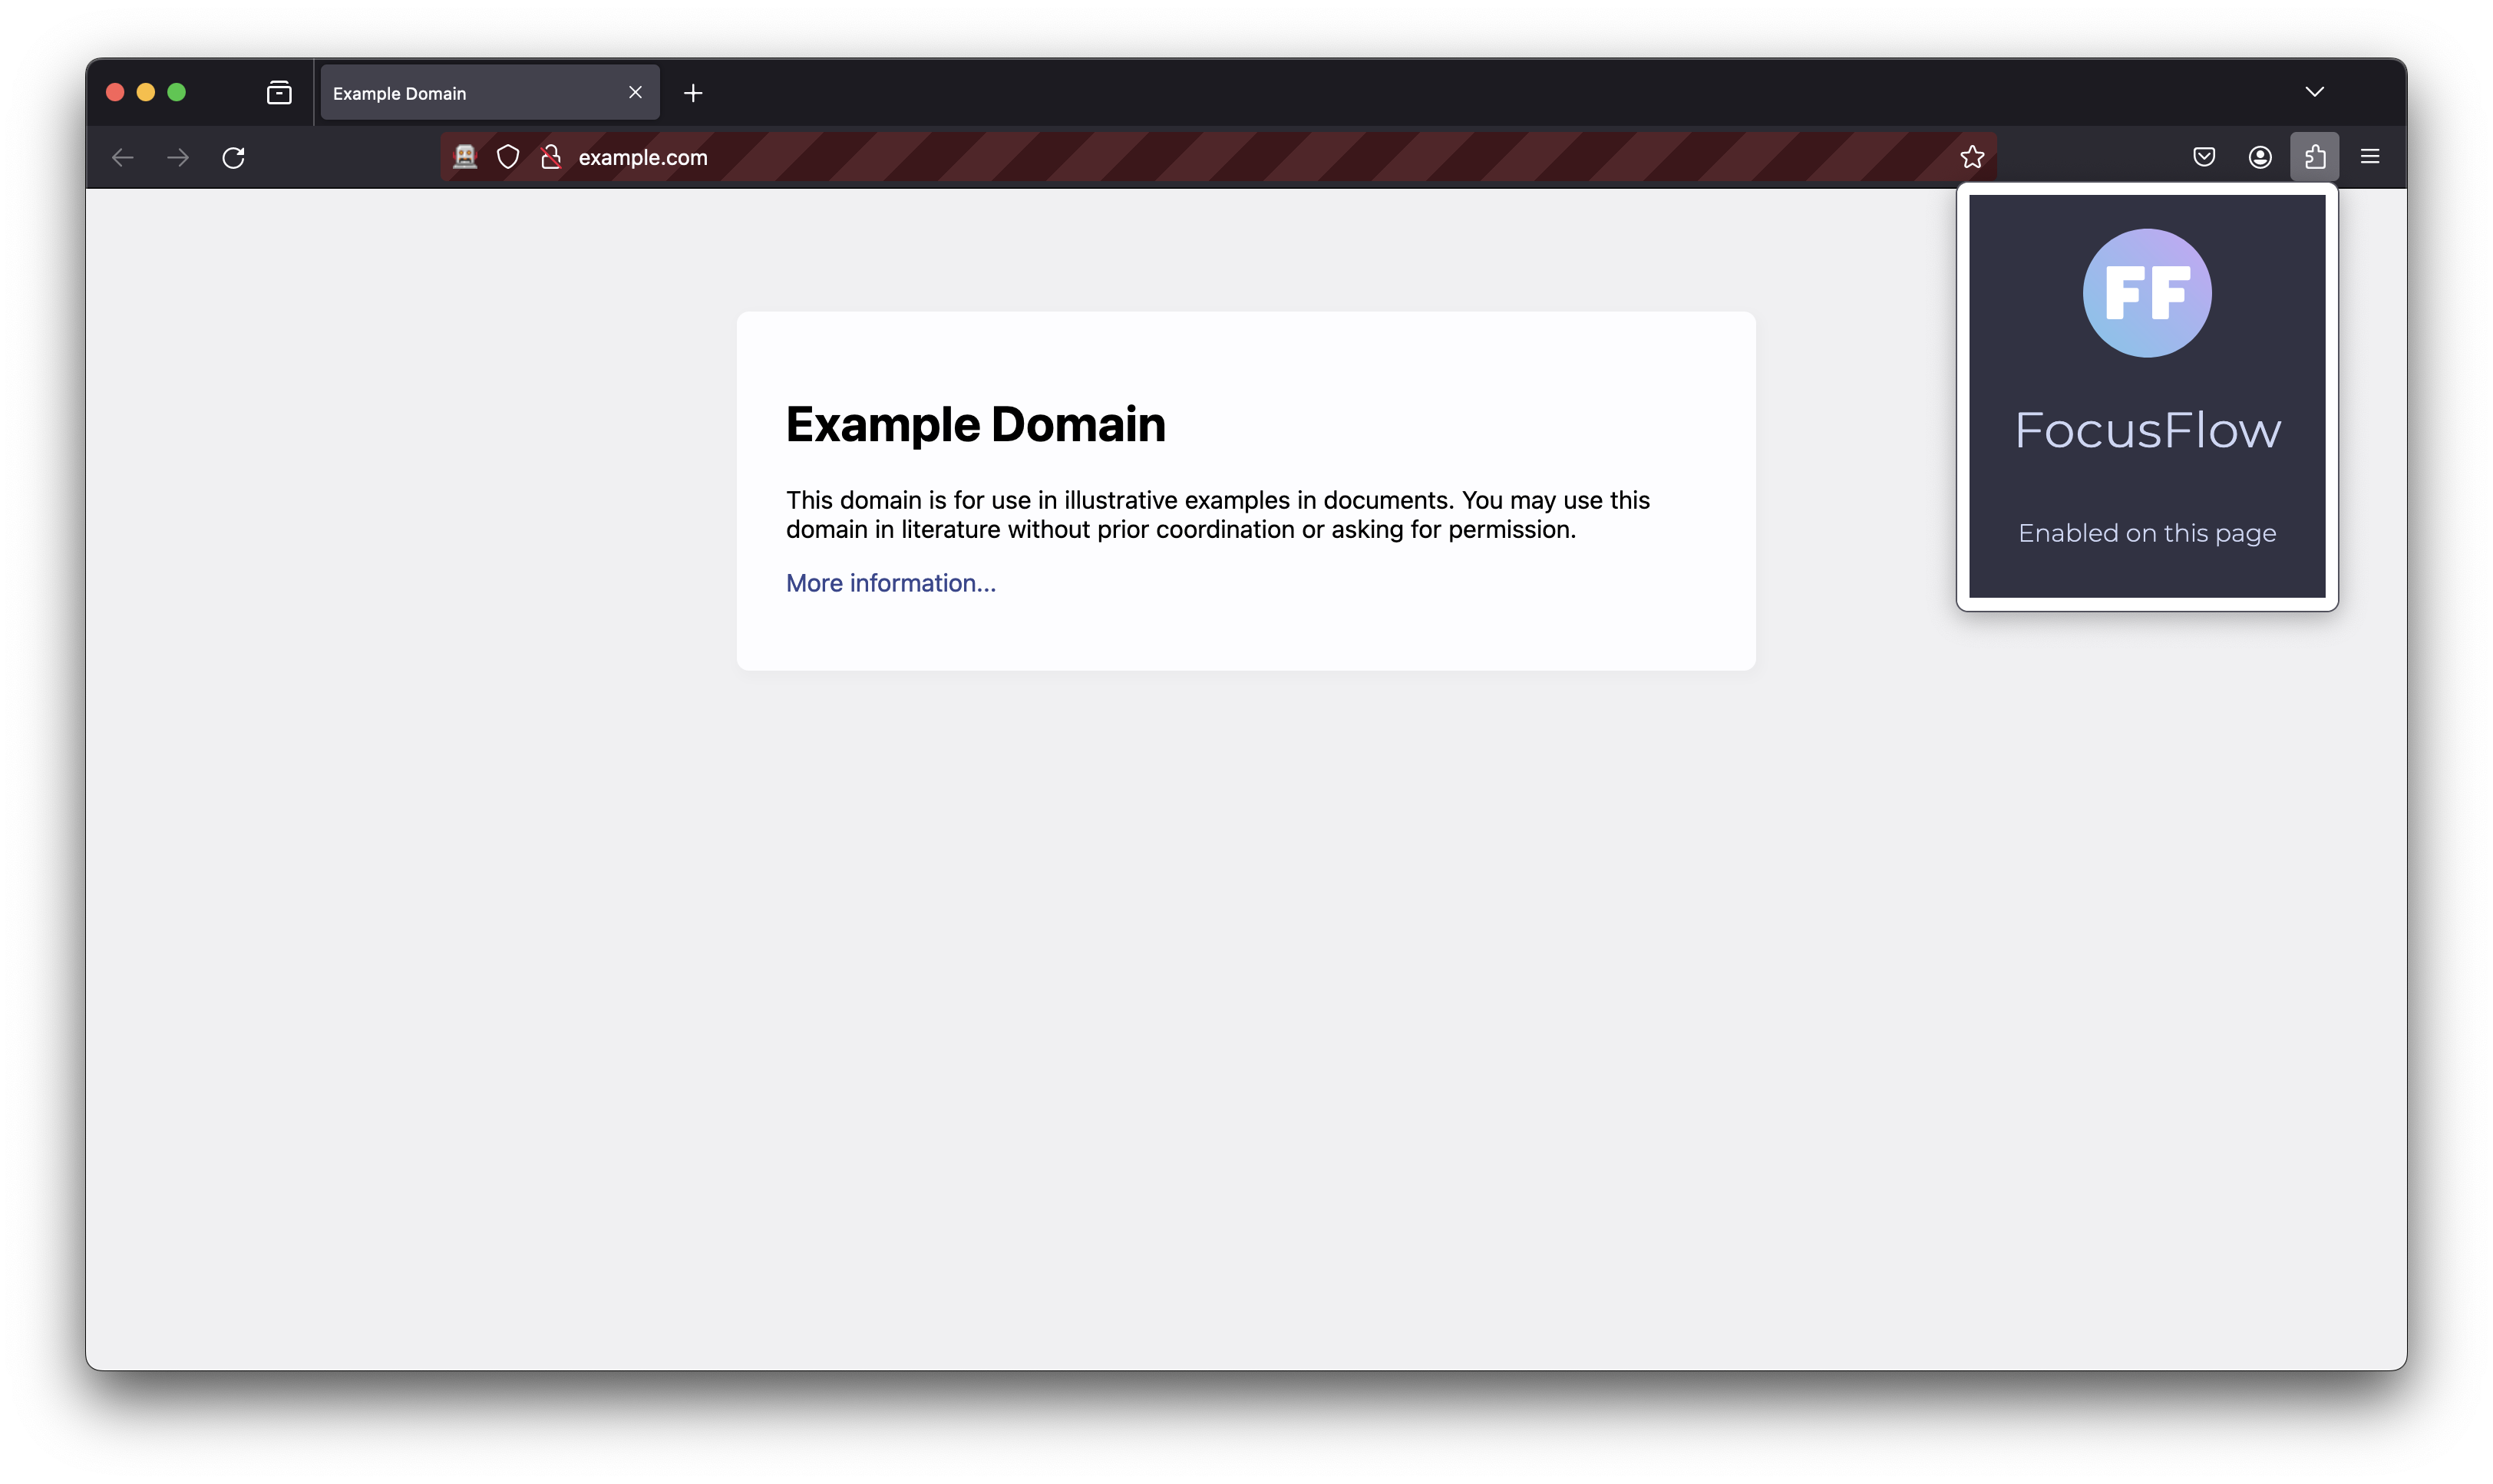
\includegraphics[width=\textwidth]{../assets/FocusFlow-firefox.png}
        \caption{The FocusFlow Browser Extension Running on the Mozilla Firefox Browser}
    \end{subfigure}
    \hfill
    \begin{subfigure}[b]{0.45\textwidth}
        \centering
        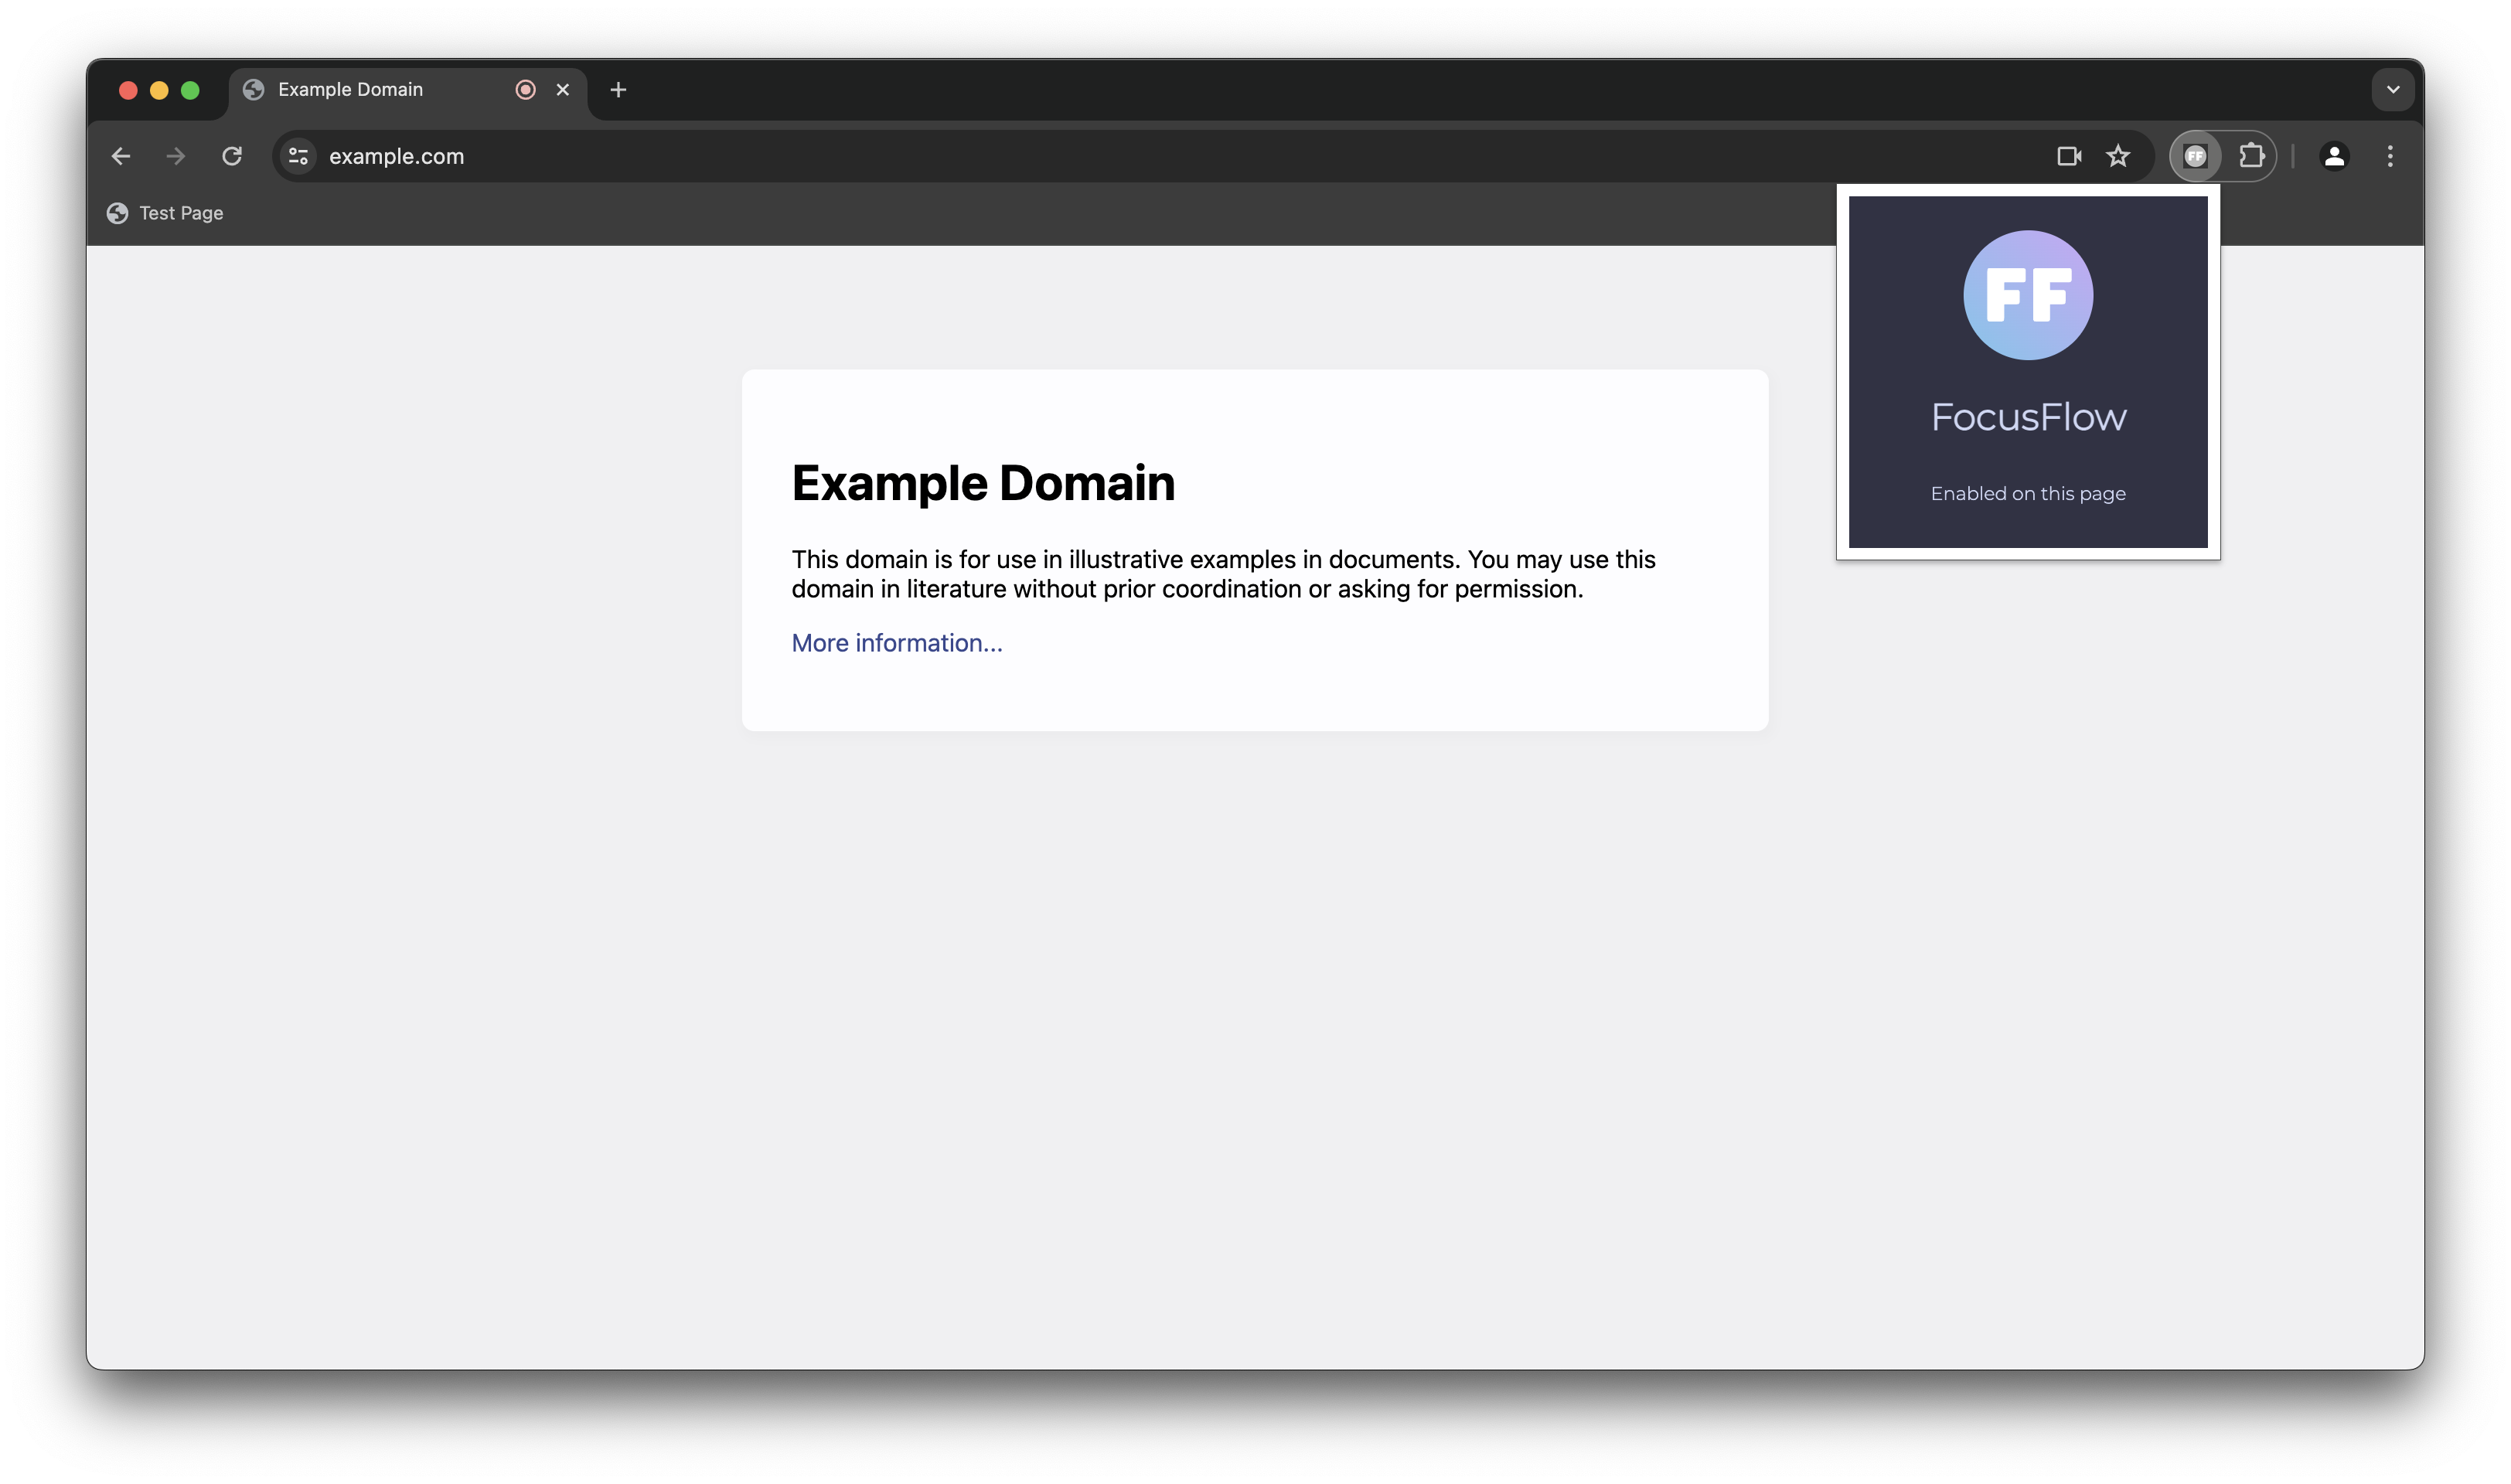
\includegraphics[width=\textwidth]{../assets/FocusFlow-chrome.png}
        \caption{The FocusFlow Browser Extension Running on the Google Chrome Browser}
    \end{subfigure}

    \begin{subfigure}[b]{0.45\textwidth}
        \centering
        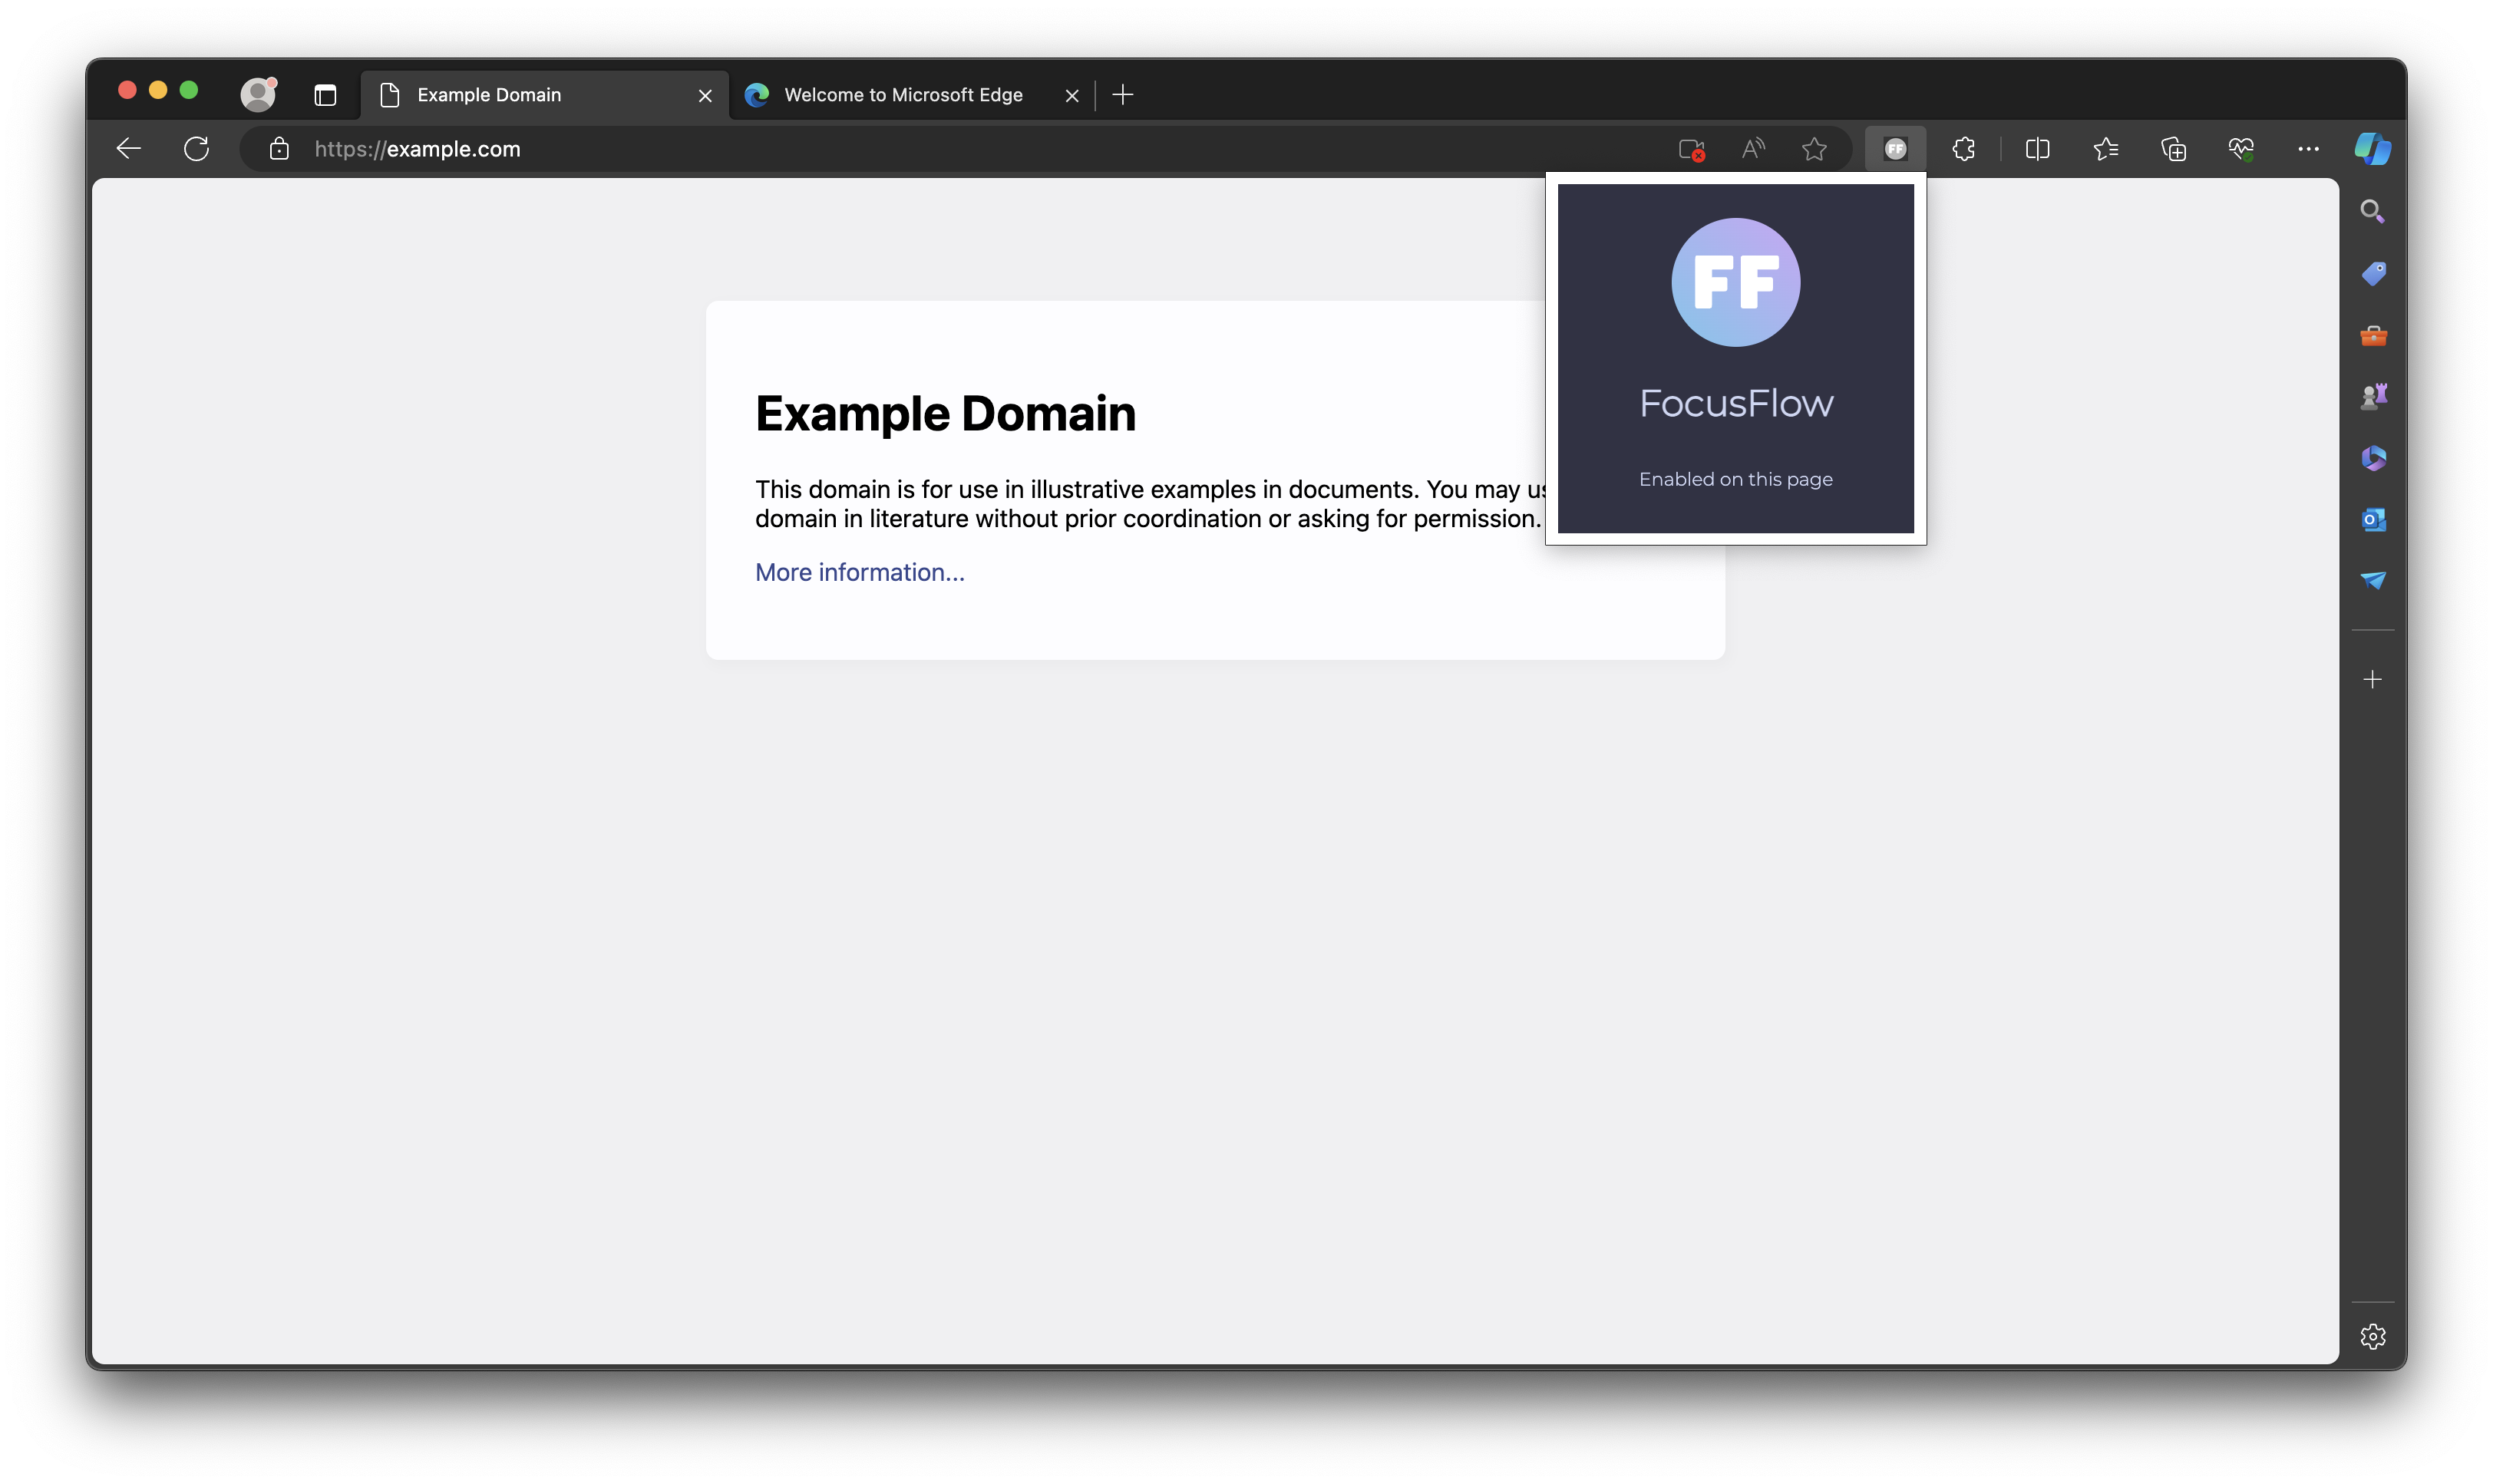
\includegraphics[width=\textwidth]{../assets/FocusFlow-edge.png}
        \caption{The FocusFlow Browser Extension Running on the Microsoft Edge Browser}
    \end{subfigure}
    \hfill
    \begin{subfigure}[b]{0.45\textwidth}
        \centering
        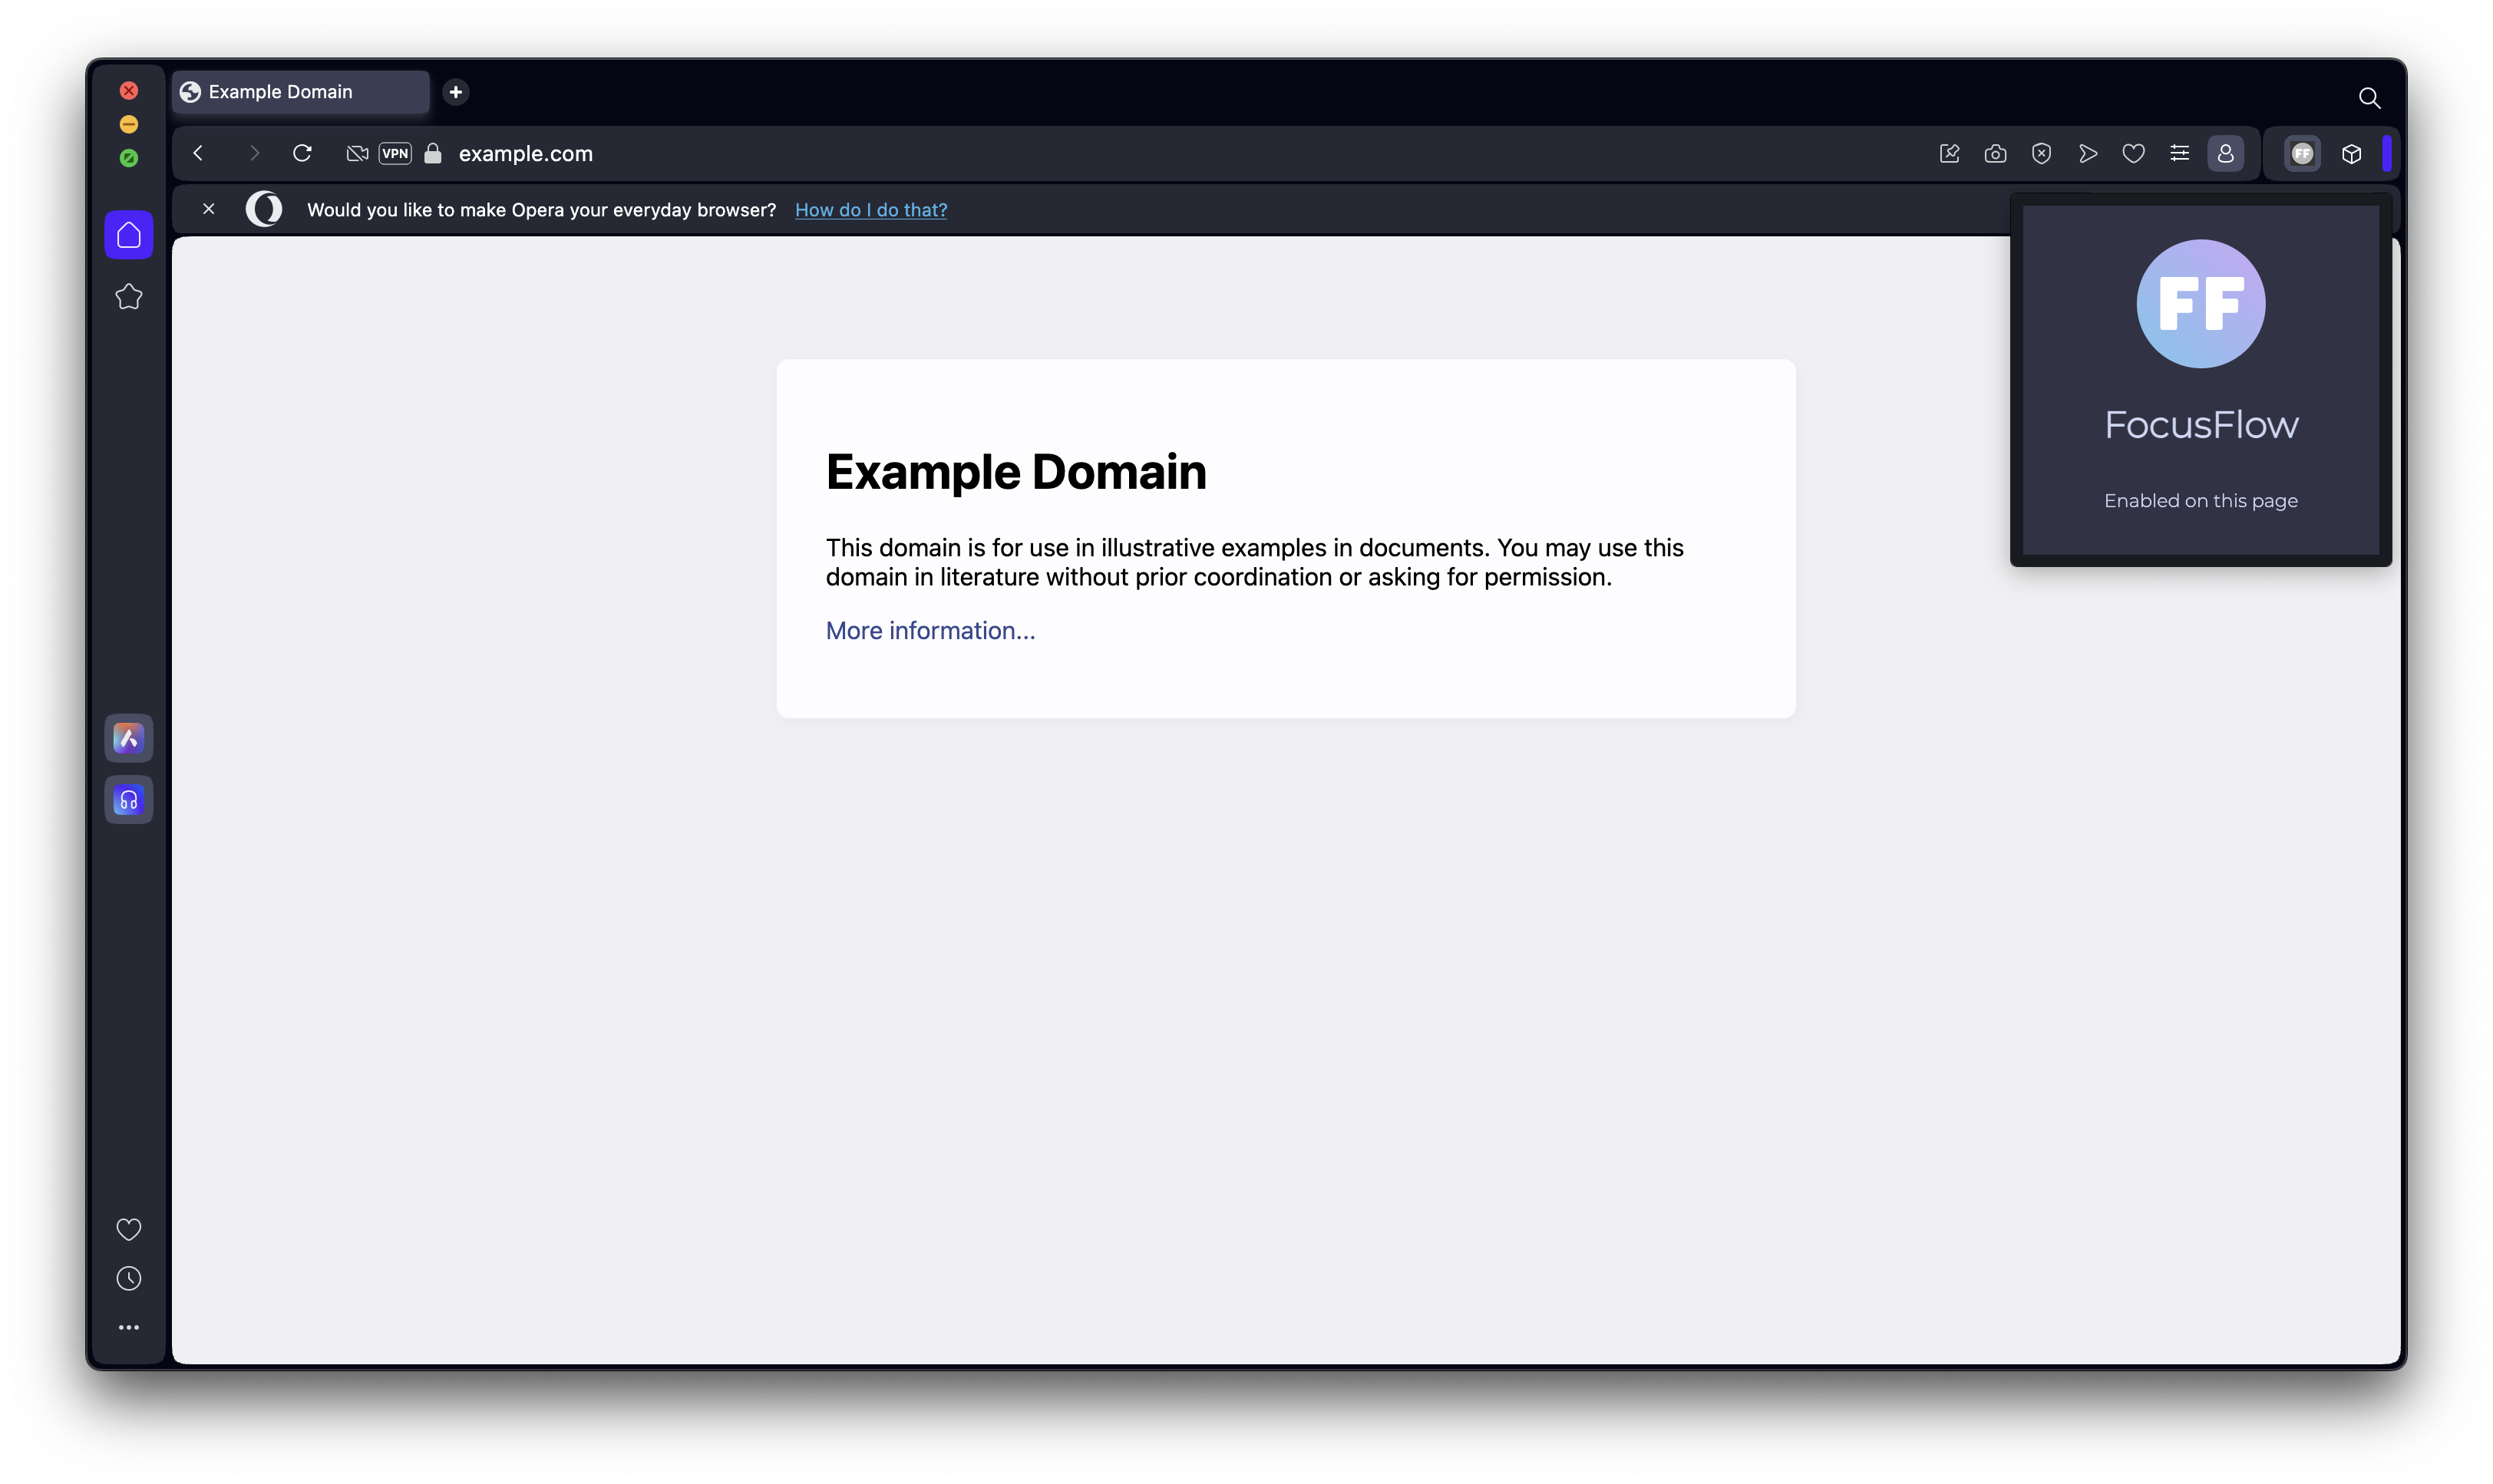
\includegraphics[width=\textwidth]{../assets/FocusFlow-opera.png}
        \caption{The FocusFlow Browser Extension Running on the Opera Browser}
    \end{subfigure}
    \caption{Browser Support For FocusFlow}
    \label{fig:browser-support}
\end{figure}


\begin{figure}
    \begin{center}
        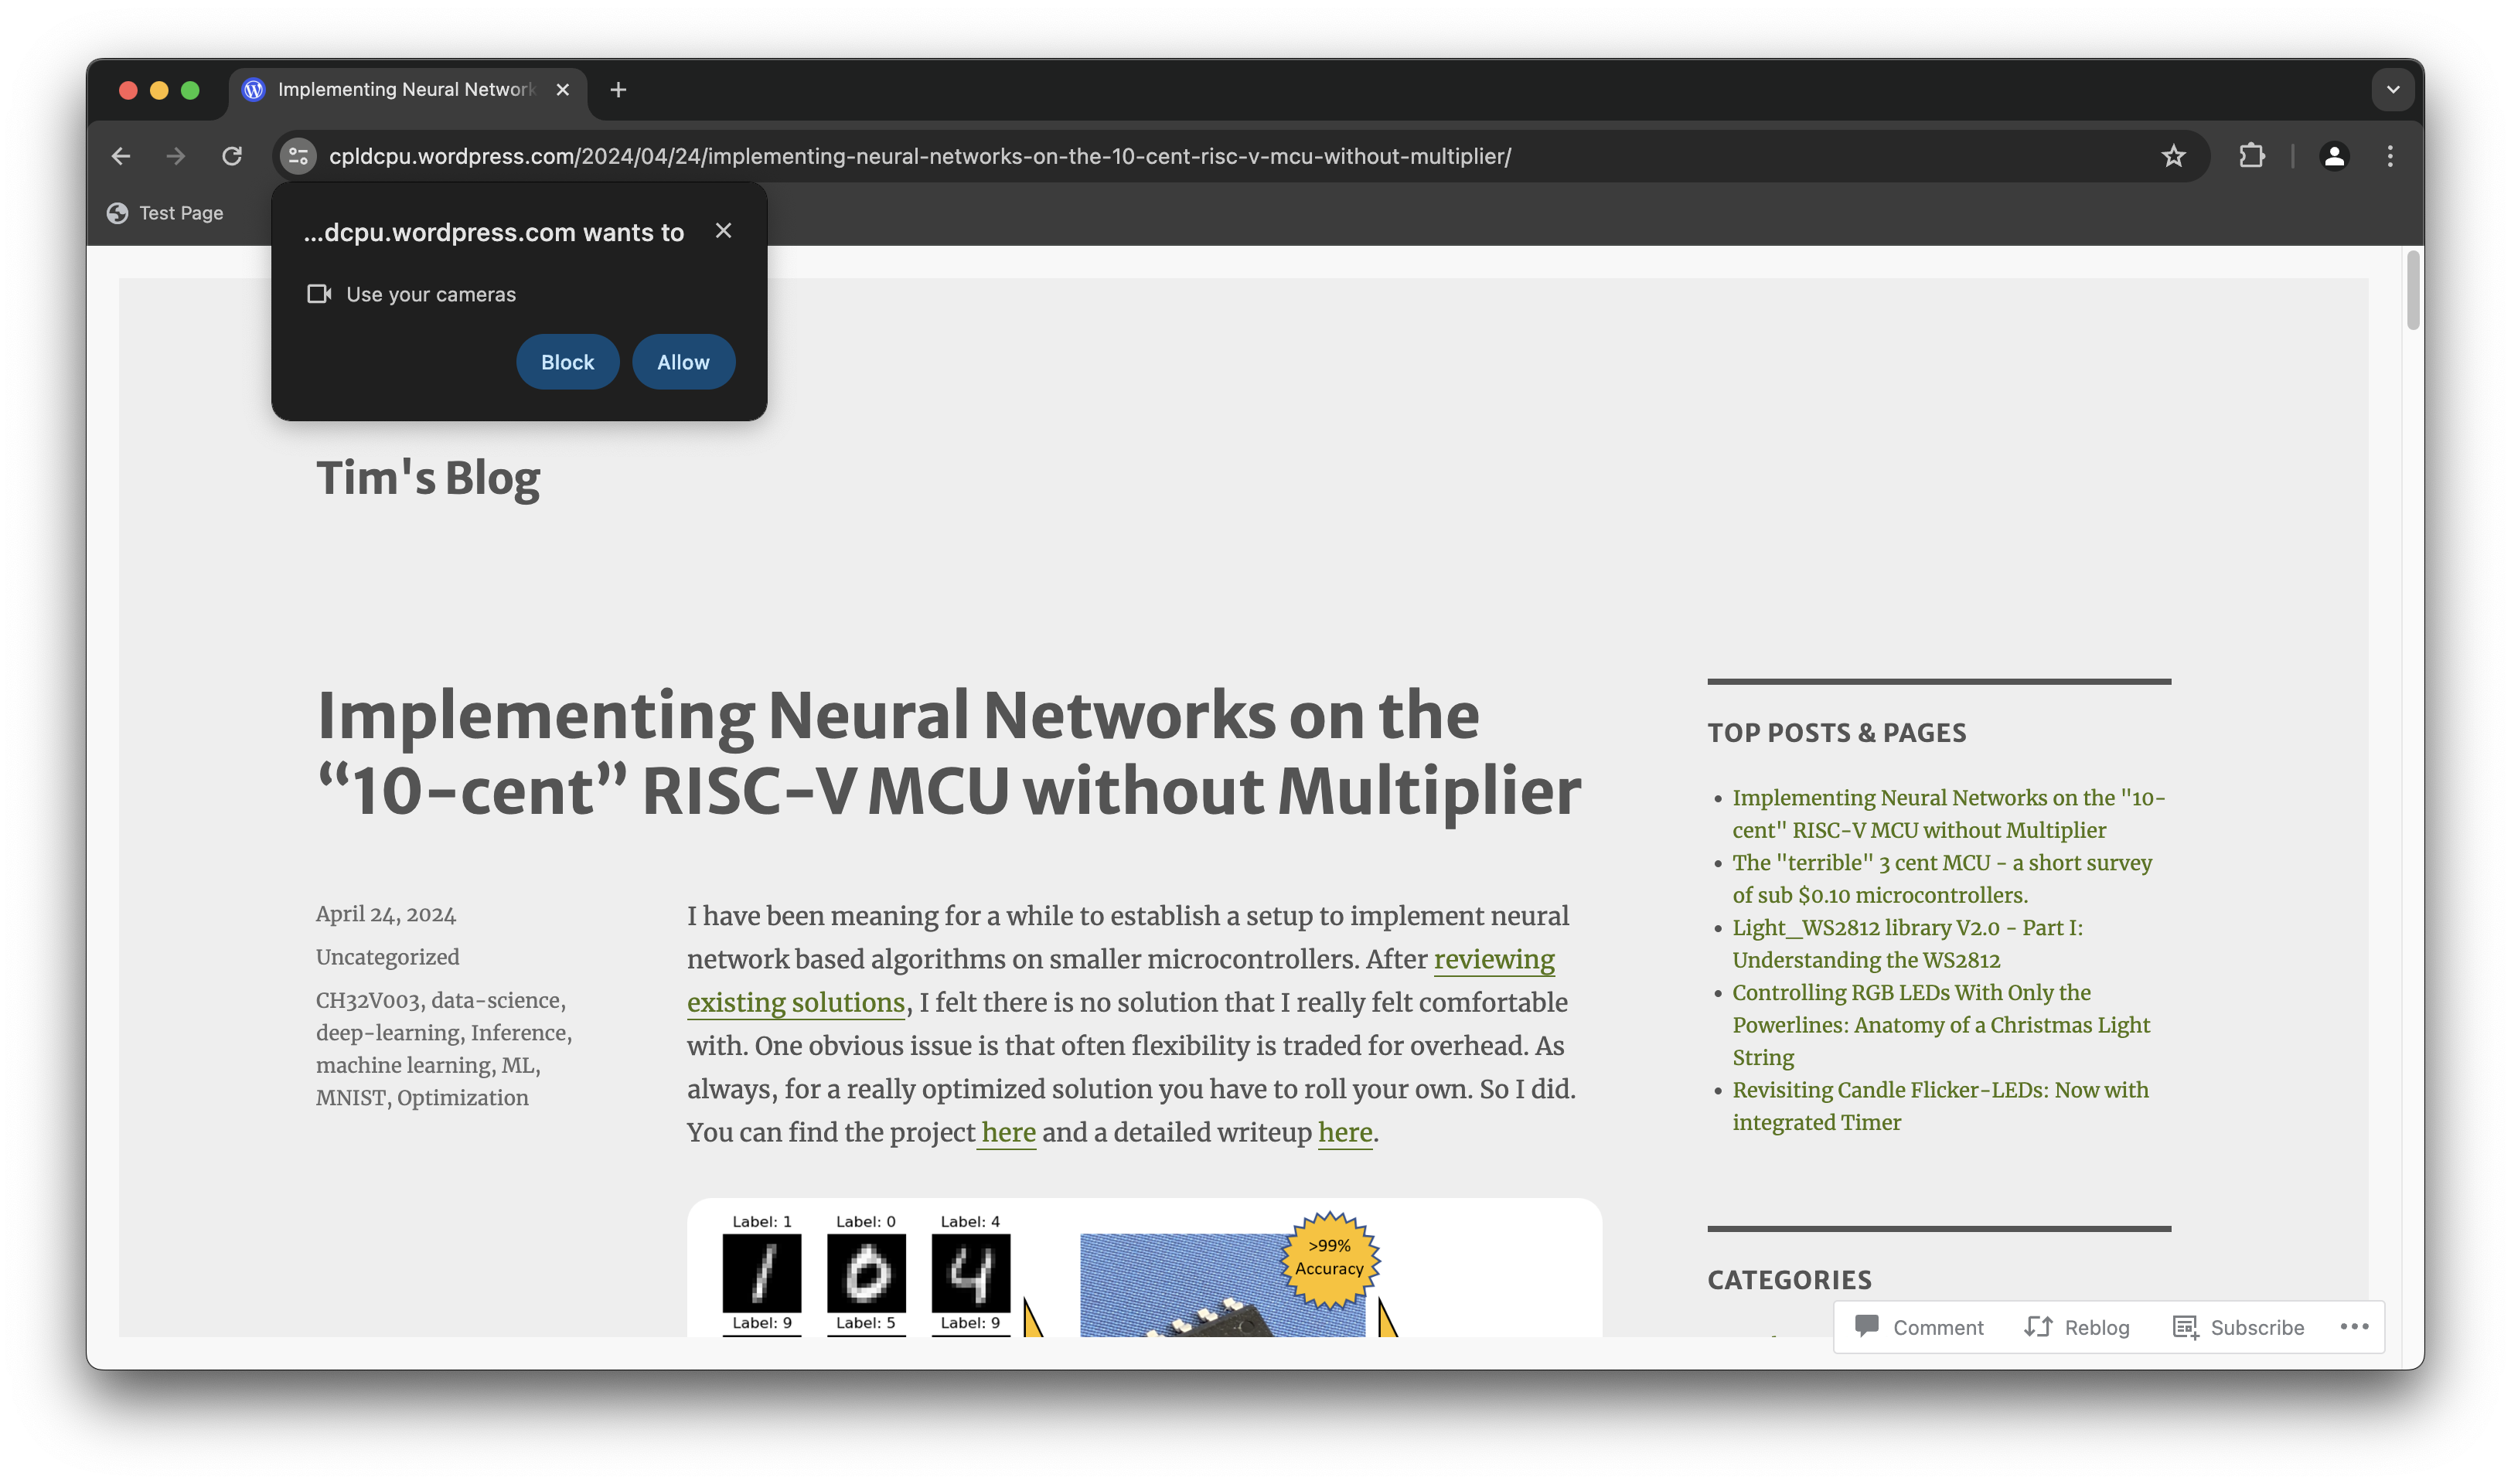
\includegraphics[scale=0.25]{../assets/FocusFlow-camera-perms.png}
    \end{center}
    \caption{FocusFlow asking for permission to use the camera before it starts tracking gaze}
    \label{fig:ff-camera}
\end{figure}

\begin{figure}[h]
    \centering
    \begin{subfigure}{0.4\textwidth}
      \centering
      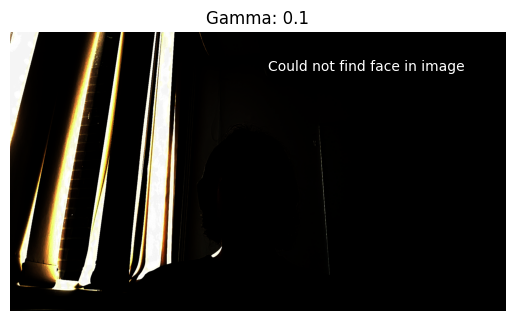
\includegraphics[width=\linewidth]{../assets/lighting-experiment/gamma-0.1.png}
    %   \caption{Subfigure A}
    \end{subfigure}%
    \begin{subfigure}{0.4\textwidth}
      \centering
      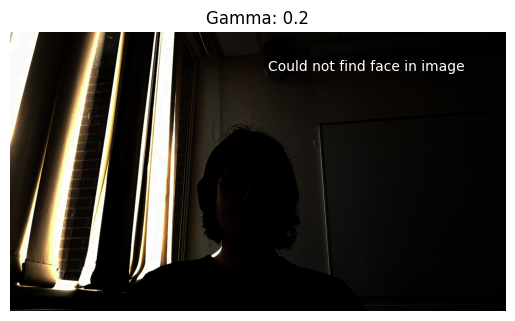
\includegraphics[width=\linewidth]{../assets/lighting-experiment/gamma-0.2.png}
    %   \caption{Subfigure B}
    \end{subfigure}\\[1em]
    \begin{subfigure}{0.4\textwidth}
      \centering
      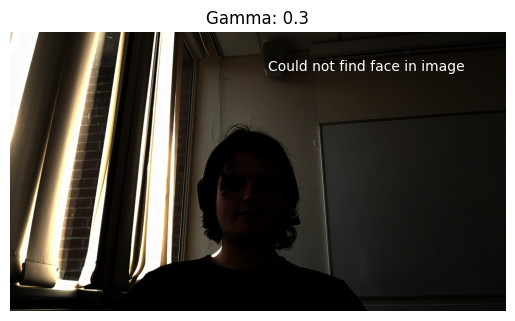
\includegraphics[width=\linewidth]{../assets/lighting-experiment/gamma-0.3.png}
    %   \caption{Subfigure C}
    \end{subfigure}%
    \begin{subfigure}{0.4\textwidth}
      \centering
      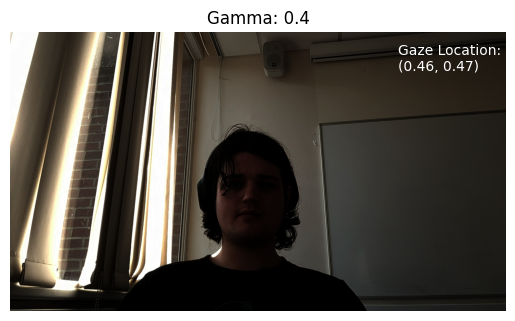
\includegraphics[width=\linewidth]{../assets/lighting-experiment/gamma-0.4.png}
    %   \caption{Subfigure D}
    \end{subfigure}\\[1em]
    \begin{subfigure}{0.4\textwidth}
      \centering
      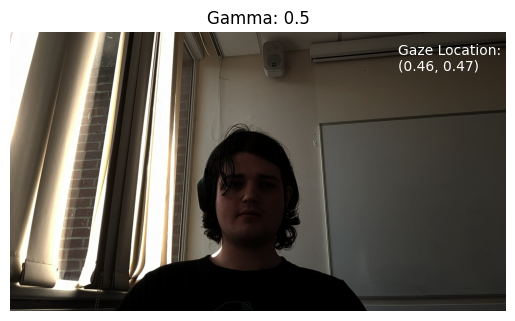
\includegraphics[width=\linewidth]{../assets/lighting-experiment/gamma-0.5.png}
    %   \caption{Subfigure E}
    \end{subfigure}%
    \begin{subfigure}{0.4\textwidth}
      \centering
      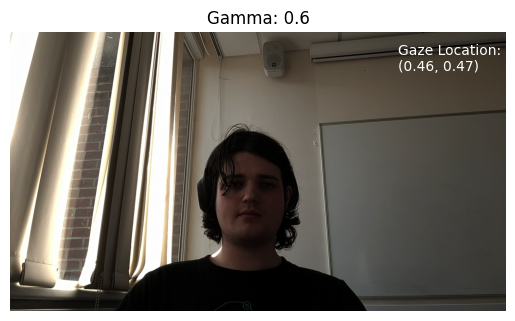
\includegraphics[width=\linewidth]{../assets/lighting-experiment/gamma-0.6.png}
    %   \caption{Subfigure F}
    \end{subfigure}\\[1em]
    \begin{subfigure}{0.4\textwidth}
      \centering
      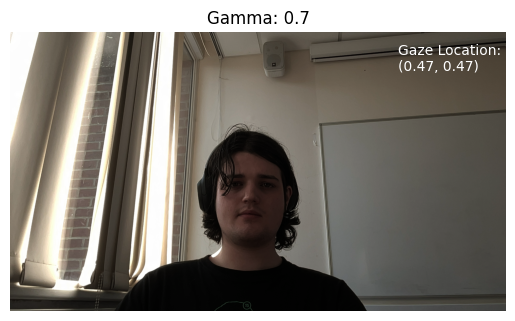
\includegraphics[width=\linewidth]{../assets/lighting-experiment/gamma-0.7.png}
    %   \caption{Subfigure G}
    \end{subfigure}%
    \begin{subfigure}{0.4\textwidth}
      \centering
      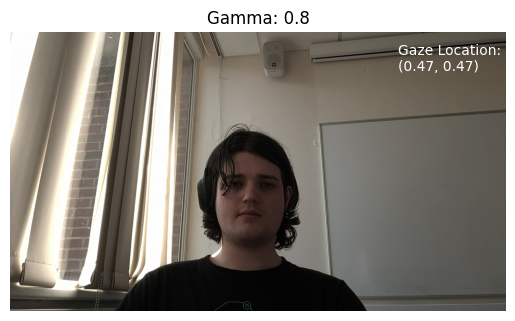
\includegraphics[width=\linewidth]{../assets/lighting-experiment/gamma-0.8.png}
    %   \caption{Subfigure H}
    \end{subfigure}\\[1em]
    \begin{subfigure}{0.4\textwidth}
      \centering
      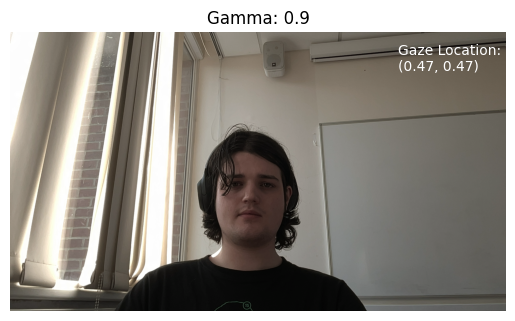
\includegraphics[width=\linewidth]{../assets/lighting-experiment/gamma-0.9.png}
    %   \caption{Subfigure I}
    \end{subfigure}%
    \begin{subfigure}{0.4\textwidth}
      \centering
      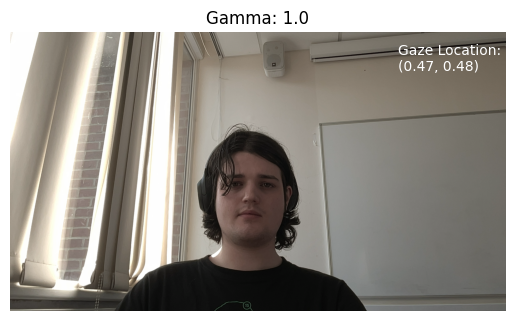
\includegraphics[width=\linewidth]{../assets/lighting-experiment/gamma-1.png}
    %   \caption{Subfigure J}
    \end{subfigure}
    \caption{Performance of the iTracker model in a variety of lighting conditions}
    \label{fig:lighting}
\end{figure}


\chapter{Discussion: Future Work}

\section{Exploring Alternative Training Datasets}

I initially planned on using 3 datasets, Gazecapture~\cite{krafka2016eye}, MPII Face Gaze~\cite{zhang2019mpii}, and ETH-X Gaze~\cite{zhang2020ethxgaze}. I initially wanted to merge each of these datasets into one large dataset which would increase the amount of data available to the model and hopefully increase its performance.

I believed merging the three datasets into one larger one would significantly increase the performance of my model as they all captured data in unique environments. Both Gazecapture and MPII Face Gaze were captured ``In-the-wild'', meaning data instances were collected in an uncontrolled environment, such as the participant's bedroom, a library or a coffee shop. This leads to the training data having a variety of lighting conditions but generally having limited variation in head pose~\cite{cheng2021survey}. This is most noticeable in the MPII Face Gaze dataset and is less of an issue in the Gazecapture dataset as subjects of this dataset were instructed to move their phone around as they completed the data collection. ETH-X Gaze however captures subjects in a controlled environment and captures 18 different angles concurrently. The authors also varied the lighting conditions when capturing data.

However, the ETH-X Gaze dataset did not include any annotations for 2D gaze targets. While I could've used the method outlined in~\cite{zhang15cvpr} to convert between a gaze direction vector and a pixel-wise gaze target, I was unable to find the time to implement this. Further work could add samples from this dataset into the training data to help the model better learn variations in both head pose and lighting conditions, despite the data being captured in a controlled setting. As the images were captured in a controlled setting, estimating the origin, and screen pose would be easier than converting 3D gaze vectors to gaze targets in an in-the-wild setting, as the origin and screen pose would be different in each instance. 

Training the model on this dataset would've also required the development of a custom data reader, which transforms the raw data into something that the model can understand. This requires the use of another machine learning model, such as the 68-point facial landmark shape predictor~\cite{king2015models} model offered by dlib~\cite{king2009dlib}, to crop certain elements of the face, such as the eyes, and face. I made use of this model as part of the REST API.

\section{Gaze Estimation Research Studies}

As explored in Section~\ref{chap:methods}, I made use of the iTracker model~\cite{krafka2016eye} to handle performing gaze location inference. This was because of its ability to learn gaze inference on images taken from a webcam or front-facing camera with very little pre-processing when compared to other models. However, further work could develop and evaluate the effectiveness of other, custom models based on state-of-the-art architectures found in the literature such as~\cite{seonwook2019fewshot,tafasca2023sharingan}. 

Further work could also research the effect of utilizing a 3D gaze vector model, such as~\cite{zaho2024gazeswin,yu2019deep} on the accuracy of the final product. I was unable to implement this myself as the process of converting between 3D gaze direction vectors requires estimating both the head pose of the user and the position of the screen within 3D space~\cite{zhang15cvpr}. However, further research could involve the prediction of these parameters. For example, making use of techniques such as Appearance template methods~\cite{niyogi1996example}, in which a new image of a head is compared to a set of examples labeled with a discrete pose to find the most similar pose, or detector array methods where a series of head detectors are trained on a specific pose and assign a discrete pose to the detector with the greatest support, among numerous other methods which are explored in~\cite{chutorian2009head}. Screen pose can be determined easily on mobile devices by making use of the gyroscopes that are present in nearly all modern smartphones. Desktop devices are less likely to have these sensors, as they are typically static while in use, which makes it far easier to estimate their pose in 3D space.

Another aspect of this project that should be explored is how well a pre-trained model performs. A variety of pre-trained models exist and have been shown to perform very well across a variety of domains within the gaze mapping field~\cite{akinyelu2020convolutional}, so it would be interesting to see if they are capable of higher accuracy than the iTracker model. This would require using any number of the existing pre-trained models such as ResNet~\cite{he2015deep}, AlexNet~\cite{krizhevsky2017imagenet}, and modifying the network architecture such that it outputs a 2D vector representing the gaze location on a screen. Then, perform transfer learning on a smaller dataset. This would cut down significantly on training time, and could also be used for calibration to improve the performance of the model. 

Another aspect that my project did not consider which would be a good area for further research could be the calibration of these models. Approaches such as FAZE ~\cite{seonwook2019fewshot} could be used to improve the performance of the final product. 

Commercial approaches such as the devices manufactured by Tobii~\cite{tobiiprofusion} could also be integrated into the software to see how a non-appearance-based approach could solve the problem. This device can reportedly achieve far higher accuracy of eye tracking to within \(\ang{0.3}\) of the true gaze vector, and it would be interesting to see whether it is capable of detecting gaze on a far smaller scale than paragraphs, such as lines or even individual words. 

As explored in the evaluation of the machine learning model,~\autoref{sec:itracker-eval}, the horizontal component of the gaze location is significantly less important than the vertical component. This is because most websites arrange text in a single-column format. Therefore, it may improve the performance of the model to disregard this component of gaze location altogether and focus solely on the vertical. This would also require modification of the browser extension to modify the bounding boxes of the paragraph elements such that they span the width of the entire page, instead of just using the bounding box provided by the \texttt{HTMLElement.getBoundingClientRect} method.


\subsection{Transfer Learning}

The two datasets I chose to use varied massively in terms of available data. MPIIFaceGaze has a total of 15 participants for a total of 45000 images, whereas Gazecapture has a total of 1474 participants with a total of 1490959 images. This made the training times for the two models drastically different, as discussed in Section~\ref{sec:training}, it took nearly 30 hours to perform 25 epochs of training on MPII Face Gaze. Using the same hardware, it would've taken nearly a month to perform a similar training run. 

For this reason, I chose to perform transfer learning on the model trained on MPII Face Gaze with a subset of the Gazecapture dataset. I chose to only modify the weights of the fully connected layer, and freeze all of the weights in the convolution layers. 

The use of transfer learning allows deep learning models to be adapted to a new domain, using a smaller dataset~\cite{koehrsen2018transfer}. 


\section{Browser Extension \& Backend API}

The API that handles gaze inference was initially going to be developed in the Rust programming language. This is because I am very familiar with this language, it's robust to memory-based bugs, and it's extremely performant due to its focus on speed while still affording developers high-level abstractions, such as its excellent type and hygienic macros systems. This was because I wanted to leave the option open to perform live gaze tracking on the webpage. This would help when considering the potential for developing accessibility browser extensions as outlined in~\autoref{ssec:stretch}, as it would have to update in real-time, likely making many inferences every second and therefore multiple requests to the API every second. Thus requiring an API with very low latency. Rust-based APIs are known to be extremely performant~\cite{ali2020benchmark}, with most REST API frameworks being capable of at least 300000 requests per second, some even reaching 500000 requests per second, whereas the Python API framework I ended up using, FastAPI, was only capable of achieving 255000 requests per second. This would probably be fine for a locally hosted API, but future work on this project could find that it would be optimal to remotely host the model instead. In this case, it would be necessary to ensure the API is as fast as possible to enable multiple, concurrent users to use the browser extension at the same time. 

In the end however, I decided to implement the API in python instead as I was unable to get the image pre-processing models to work in rust. While multiple libraries exist for this purpose, they are not compatible with the format the dlib facial alignment model~\cite{king2009dlib} is released in, and a Foreign Function Interface (FFI), which would allow me to call C and C++ functions from rust, is not available for the dlib C++ library, meaning I would have to implement it myself. While rust makes it easy to develop FFIs, I am not experienced with this, and I could not find the time to develop the skills necessary, opting to instead use Python as the developer experience to get everything working was far easier due to the existence of libraries for interacting with the dlib models.

\chapter{Conclusion}

% \nocite{*}
\printbibliography

\appendix 

\chapter{Project Log}

\begin{itemize}
    \item 2023-06-02 Begun preliminary reading 
    \item 2023-08-01 Begun work on web extension 
    \item 2023-08-02 Looked at other peoples implementations of gaze mapping software \& tried item to detect paragraphs in the viewport on a webpage 
    \item 2023-08-03 Performance improvements to paragraph detection on webpage 
    \item 2023-08-06 Changed how paragraph detection works 
    \item 2023-08-07 Started work on my own model for gaze mapping 
    \item 2023-08-20 Migrated browser extensions to Plasmo framework 
    \item 2023-09-12 Tried to build a dataset loader, encountered difficulties as I haven't been given ethical approval to use datasets yet, so I'm basing it off the description of the dataset
    \item 2023-09-20 Sent an email to Temitayo, regarding potentially acting as my supervisor
    \item 2023-09-22 Did some more reading \& work on ethics application  
    \item 2023-09-25 Spoke to Temitayo about project proposal, discussed the need for an
    \item ethics application, agreed to act as my supervisor 
    \item 2023-10-02 Meeting with Temitayo about the ethical application, shared feedback on my application 
    \item 2023-10-11 Started on interim report 
    \item 2023-10-20 Tried to get iTracker model to train on my local machine using a small custom dataset 
    \item 2023-10-31 Submitted ethics application \& ethics application returned for revision
    \item 2023-11-08 Submitted revised ethics application 
    \item 2023-11-13 More work on interim report, includes more background reading 
    \item 2023-11-27 Approval received from ethics department, browser can now detect visible elements on the page, detects webpage going in/out of focus. Looked at a number of existing eye tracking models   
    \item 2024-01-18 Developed a program to crop eyes, face and to produce a binary mask for pre-processing 
    \item 2024-01-25 Begun work on the API hosting the machine learning model, sent out revised ethics application 
    \item 2024-02-01 Training itracker model on mpiifacegaze model, browser extension now highlights an element on the page 
    \item 2024-02-08 Plan for literature review, tried merging gazecapture and mpiifacegaze datasets, recieved revised ethics application. 
    \item 2024-02-19 Debugging session with my supervisor to figure out an issue with the length of time required to perform validation, made a plan for testing the final product, review of existing literature 
    \item 2024-02-29 Finished development of the API 
    \item 2024-07-03 Wrote outline for the report
    \item 2024-04-01 Trained iTracker on MPIIFaceGaze for 25 epochs, performed data augmentation on the MPII Face Gaze dataset to normalise the locations of gaze, started work on final report, finalized the codebase 
    \item 2024-05-01 Finished report \& made a demonstration video 
    
\end{itemize}

\end{document}